%%%%%%%%%%%%%%%%%%%%%%%%%%%%%%%%%%%%%%%%%%%%%%%%%%%%%%%%%%%
% EPFL report package, main thesis file
% Goal: provide formatting for theses and project reports
% Author: Mathias Payer <mathias.payer@epfl.ch>
%
% This work may be distributed and/or modified under the
% conditions of the LaTeX Project Public License, either version 1.3
% of this license or (at your option) any later version.
% The latest version of this license is in
%   http://www.latex-project.org/lppl.txt
%
%%%%%%%%%%%%%%%%%%%%%%%%%%%%%%%%%%%%%%%%%%%%%%%%%%%%%%%%%%%
\documentclass[a4paper,11pt,oneside]{report}
% Options: MScThesis, BScThesis, MScProject, BScProject
\usepackage[MScThesis,lablogo]{EPFLreport}
\usepackage{amsmath,amssymb,amsthm} % math typesetting
\usepackage{dsfont} % for indicator function
\usepackage[utf8]{inputenc}
%\usepackage{natbib} % how to make it work???
\usepackage{xspace} % possibly add space after something
\usepackage{hyperref} % autoref and WEB URLs
\usepackage{graphicx} % figures
\usepackage{todonotes} % notes used when writing the draft
\usepackage[autostyle=try, english=american]{csquotes}


%ALternative explantion: best reparametrization of differential equations that makes the equation most simple
%DiffEquation environment+, gw env+
% IIT similar -- dynamical system, interventions on the graph
% try nonlinear ICA for ve5?
%Nonlin ICA would work for vector increment,
% finish mendeley overview, try approaches (lagrange multi+, proj <= n and dn/dt, time-scale Stackelberg_competition+, proximal sparsity)
%But it is likely to fail for sparsemateix with a linear encoder
%Add vectorinctement where the component is defined by a separate digit that is incremented and decremented using a special counter
%Implement a simpler grifworod with 2 coordinates. Try the method. If it doesn't work, why? If it does, what's the difference with keychest?
%Maybe highdim keychest would actually work better because of better disentanglement?
% complex matrix -> diagnonalizable?
% batchnorm prevents loss->0
% very slow even on linear -- trying with larger time-scale sep

% ISSUE: probas don't go down/up as they should have been -- why??
% maybe some bug in the coefficients / losses
% gw(5x5, 2feat) solved!
% sm5(noact/act) solved!
% sm5_linear(act) ...
% ve5_obs ...
% 5x5_kc_onlycoord...
% 5x5_kc_full ...

% lagrange|gap|discrete|sparsity|smooth|constraint

% ReLU is generally pretty bad and noisy

% do nonlinear ICA after handing in the report

\newtheorem{example}{Example}[section]
\newtheorem{proposition}{Proposition}[section]


\newcommand{\sysname}{CauseOccam\xspace}
\newcommand{\var}{\mbox{Var}}
% CausalOccam
% SimpleCause
% BayesianCause
% TLDRCause

\title{\sysname: Learning Interpretable Abstract Representations in Reinforcement Learning Environments via Model Sparsity}
\author{Sergei Volodin}
\supervisor{Dr. Johanni Brea}
\adviser{Prof. Wulfram Gerstner}
%\coadviser{Second Adviser}
\expert{Carl-Johann Simon-Gabriel}

\dedication{\begin{raggedleft}
        The strongest evidence that we can obtain for the validity of a proposed induction method, is that it yields results that are in accord with intuitive evaluations in many different kinds of situations in which we have strong intuitive ideas.\\
        --- Ray J. Solomonoff\\
    \end{raggedleft}
}

\acknowledgments{
I thank my parents and my sister for the support in my studies, and Switzerland and EPFL in particular for making it possible.

I would like to also thank Nevan Wichers, Le Nguen Hoang, El-Mahdi El-Mhamdi, Louis Faucon David Krueger, Ivan Vendrov, and Jeremy Nixon for the productive discussions in 2019-2020 on Causality and Machine Learning in general.

I would like to additionally thank Roman Pogodin for introducing me to EPFL and to computational neuroscience. I would like to thank Konrad Seifert, Mattias Berg, Ailin Parsa, Romain Ensminger, Denis Drescher, Michael Pokorny for supporting me.

Special thank you to my supervisor Johanni Brea for guiding and supporting me during the thesis.

}

\address{EPFL IC/SV Laboratory of Computational Neuroscience (LCN)\\
    Bâtiment AAB \\
    offices 135-141 \\
    CH-1015 Lausanne}

\begin{document}
    \maketitle
    \makededication
    \makeacks

\begin{abstract}

"I choose this restaurant because they have vegan sandwiches" could be a typical explanation we would expect from a human. However, current Reinforcement Learning (RL) techniques are not able to provide such explanations, when trained on raw pixels.
RL for state-of-the-art benchmark environments are based on neural networks, which lack interpretability, because of the very factor that makes them so versatile -- they have many parameters and intermediate representations.
Enforcing safety guarantees is important when deploying RL agents in the real world, and guarantees require interpretability of the agent.
%The best result that could be obtained are two rollouts from the internal model of the agent, showing that one policy would result in a higher reward than the another policy. These rollouts would be high-dimensional objects that are hard to compare together or reason about.
%Additionally, feature attribution could be applied to these rollouts, which would show that certain parts of the raw image observations influence the outcome more than others. However, this would require a careful manual analysis of the feature attribution maps for every possible input that the agent can encounter.
Humans use short explanations that capture only the essential parts.
%This is possible because the world contains hierarchical structures in which only a few factors are important, and the rest can be ignored.
In our thesis, we address the problem of making RL agents understandable by humans.
%Interpretability of the resulting agent is crucial if such an agent is deployed in the real world in mission-critical scenarios, because a black-box neural network could give wrong predictions on unexpected inputs, without even giving an ability to know the reason of the failure. Thus, interpreting Reinforcement Learning agents is an important step towards safely deploying them.
In addition to the safety concerns, the quest to mimic human-like reasoning is of general scientific interest, as it sheds light on the easy problem of consciousness.

%To make an agent that can reason like a human does, we first need to learn a representation that corresponds to high-level objects contained in the environment, and their properties, like the representation that the natural language uses.
The problem of providing interpretable and simple causal explanations of agent's behavior is connected to the problem of learning good state representations.
If we lack such a representation, any reasoning algorithm's outputs would be useless for interpretability, since even the "referents" of the "thoughts" of such a system would be obscure to us.
%: it would take many words of natural language to explain one concept that the system uses.
% Thus, a subgoal of making interpretable agents is to create representations that allow for simple explanations of causes and their effects in a given environment.

One way to define simplicity of causal explanations via the sparsity of the Causal Model that describes the environment: the causal graph has the fewest edges connecting causes to their effects. For example, a model for choosing the restaurant that only depends on the cause "vegan" is simpler and more interpretable than a model that looks at each pixel of a photo of the menu of a restaurant, and possibly relies as well on spurious correlations, such the style of the menu.

%In addition, sparse causal models describing the latent dynamics are hypothesized by Yoshua Bengio to be crucial in the functioning of human consciousness, since human explanations have only few important causes.

In this thesis, we propose a framework \sysname for model-based Reinforcement Learning where the model is regularized for simplicity in terms of sparsity of the causal graph it corresponds to.
The framework contains a learned mapping from observations to latent features, and a model predicting latent features at the next time-steps given ones from the current time-step. The latent features are regularized with the sparsity of the model, compared to a more traditional regularization on the features themselves, or via a hand-crafted interpretability loss.
To achieve sparsity, we use discrete Bernoulli variables with gradient estimation, and to find the best parameters, we use the primal-dual constrained formulation to achieve a target model quality.
The novelty of this work is in learning jointly a sparse causal graph and the representation taking pixels as the input on RL environments.
We test this framework on benchmark environments with non-trivial high-dimensional dynamics and show that it can uncover the causal graph with the fewest edges in the latent space.
We describe the implications of our work to developing priors enforcing interpretability.

%For the future work, the causal graph can be used for easier grounding on a set of natural language explanations, as the agent now "knows" about the high-level concepts that the environment contains. In addition, a simple model would likely be less prone to overfitting, which could result in an improved robustness of such agents to distributional shift.
\end{abstract}

\maketoc

%%%%%%%%%%%%%%%%%%%%%%
\chapter{Introduction}
\label{ch:intro}
%%%%%%%%%%%%%%%%%%%%%%

Reinforcement learning is a general paradigm in Artificial Intelligence (AI) that considers two entities: an environment and an agent which interact with each other over multiple time-steps. The agent takes actions in the environment, and the environment gives the agent an observation representing the state of the environment, and a reward. The goal of the agent is to execute actions that lead to highest total reward during the interaction.

While RL environments in general can have arbitrary complexity, practically interesting environments usually have a certain low-dimensional structure in them. For example, in the popular CartPole environment, the observation (as image) has 720 000 variables, while the dynamics of the cart can be explained using only 4 variables with a simple Newtonian update rule. Atari games, while having 100 800 variables in an observation, can be described using only 128 bytes (of the RAM state). The dynamics in the pixel space would be complex, with one pixel at the next time-step potentially depending on all of the pixels on the previous one. However, the dynamics in the latent space is much simpler. The real world has this property as well: while a camera can capture many megapixels per second observing a drone, the equations describing the dynamics of the drone only have a few variables, and are much simpler.


RL agents could (and sometimes already do) solve real-world problems, such as steering the wheel of an autonomous car, controlling a plant, or determining which content to recommend to people on a social network. However, in many applications there exist highly undesirable outcomes, such as the car crashing due to a mistake in controlling it, or showing polarizing or controversial content to people. To prevent such cases, we need to have an understanding of what makes an agent take a certain action, why it "thinks" it is optimal, and why it "thinks" it does not violate any sensitive constraints. Since the most capable agents are based on neural networks (NNs), it is hard to interpret them. Both the large number of parameters in the network, and many intermediate representations at each layer -- the distinctive features that allow NNs to be so versatile in fitting different kinds of data, lead to problems with interpretability (or explainability), because apriori there is no structure in the network: all variables depend on all variables of the input.

Even the state-of-the-art approaches that look at individual neurons and try to determine their functions (such as a neuron responding to the images of dogs) do not allow to obtain a concise explanation, since, while some neurons are more important than others in predicting a particular outcome, all neurons contribute a non-zero amount to the outcome. Because of this, it becomes impossible to determine in advance what the outcome of a network would be in all of the input scenarios.

In order to make an agent interpretable (be able to answer questions of the form "why an action was taken given a particular observation"), the agent needs to grasp the high-level concepts and objects contained in the environment. This is a Representation Learning task, with an objective of obtaining representations allowing for good explanations. In addition, regardless of the task the agent is solving, it has to be able to explain in simple terms the effects of its actions on the environment.

While deep neural networks allow to fit various kinds of data, but lack interpretability due to the large number of parameters, in contrast, traditional ("good-old-fashioned" or GOFA) Artifical Intelligence (AI) approaches are interpretable (explainable) but lack the versatility of neural networks: they are not applicable to all the tasks.
Such GOFA approaches are characterized by discrete symbols that are the basis of a reasoning system, i.e. first-order logic.
These symbols correspond to real-world concepts and objects, such as the coordinates of a robot on the floor.
The drawback of such systems is that the mapping from real-world "messy" data (e.g. images from a camera) to discrete symbols (e.g. the coordinates) is hand-designed and thus requires effort.
Unifying these two approaches yields the best of both worlds, with the versatility of deep AI in being able to fit almost any dataset and the explainability of traditional AI.
To do so, we learn the representation of observations using a deep network. These representations are used by a system involving discrete components to make explainable predictions about the environment.

The quality of explanations given by such an agent would depend on the learned representation. Specifically, a representation of the observation in which every variable depends on every variable would be practically useless: an action potentially changes all of the variables, and, therefore, an explanation of action's effect would require to list all of them. Since the length of an explanation is crucial, the effect of an action should be describable by a change in only a few variables.

The current explainable RL agents can be classified into three following categories. First, many projects learn sparse representations in terms of the feature vector sparsity: the predicted learned features associated with an observation are sparse at each time-step as a vector. Such a condition, however, is neither necessary nor sufficient for the {\em explanations} of the dynamics to be simple. Indeed, any sparse coding technique will yield sparse feature vectors (for example, by assigning the first $k$ most sparse vectors to all the $k$ states of the MDP in case of a finite MDP), but a feature at the next time-step would depend on many features at the previous time-step. Indeed, without any assumption on the way the sparse features are obtained, two neighboring states can have drastically different representations. Thus, an action potentially changes all of the variables. This demonstrates that sparse feature vectors are not sufficient to have simple explanations. On the other hand, it is possible to have simple explanations without sparse feature vectors. Indeed, the state of a CartPole environment has all of the components being non-0 most of the time, and, yet, these components comply with a simple explainable kinematics equation. Thus, sparse feature vectors are not necessary for simple explanations.

Secondly, feature attribution is applied to the convolutional networks representing policies, and the analysis of circuits of the network is performed. This approach gives a) the parts of the image most relevant to predict the action and b) the visualization of what each neuron in the network is activated with. While such an approach is extremely robust to the type of the underlying agent (the analysis is performed after the training and does not require any changes in the architecture), the drawback is that it should be performed for every input image: we do not know how a particular new image would affect the outputs, since each output action still depends on all of the pixels.

Finally, a line of work is investigating {\em causal} explanations of the agents' actions. This means that a causal graph corresponding to the environment is obtained, and an explanation for an action is then a simple path-finding from the action node to the reward node in this graph. The drawback of the current projects is that the graph is either given manually (by hand), or learned with significant manual work, such as designing the feature space. In this project, we extend this line of work by making the graph learnable end-to-end from the raw observations.

We would like to automatically uncover the simple structure in the underlying complex high-dimensional observations that the environment dynamics generates -- uncover the succinct "laws of physics" that the environment operates with.
This would make the actions of an agent explainable.
It makes the actions of the agent explainable in terms of the "laws of physics" that we learn. In terms of Model-Based RL (an RL agent equipped with a model of the environment), we would like to learn a simple model of the environment.
Specifically, we would like each variable in the model to depend on the fewest possible variables at the previous time-steps. This would make actions explainable in terms of the variables an action changes, and the explanation would be short. The model is the "good-old-fashioned" component, since it includes discrete elements: the variable's causes consist of a set of elements, rather than an array of numbers of weights for all possible causes.
Mathematically, we require sparsity of the model's graph of dependencies -- the predicted output for a variable depends only on a few variables at the previous time-step. If represented as a graph (with cause-variables at the current time-step as parents and effect-variables at the next time-step as children), this graph needs to have fewest possible edges.

To allow for such a simple {\em model}, we need to change the representation, from raw high-dimensional observations to the features, which the model predicts for the next time-step. Such features are obtained from a deep learning {\em decoder}\footnote{We call it a decoder rather than an encoder because the observations are already {\em encoded} by the function mapping the simple environment states such as the cart's position and velocity into the high-dimensional observation}, a function mapping observations to features. Given a decoder, the model can be obtained by simply fitting it in a supervised way, and only selecting the cause variables that lead to an improvement in the loss. Therefore, the decoder determines the simplicity of the model.

Thus, the decoder needs to be trained jointly with the model, and it is indirectly regularized by the model: the model is directly regularized for sparsity (in terms of the number of edges), and the decoder needs to output data that such model can predict.
In our approach, the decoder is a neural network, and a model is also a neural network with a special mechanism to enforce the sparsity of the architecture.

If the the decoder is not additionally regularized for non-degeneracy, it is possible for the system to always predict constant features. This correspond to closing eyes and "predicting" successfully that everything that follows will be dark. The decoder needs to preserve the information that is relevant to the task the system is required to solve. Both in the real world, and in games, not all parts of the observations need to be predicted to achieve goals. For example, the color of an obstacle that a robot encounters is likely not important when it comes to avoiding it. However, this is task-specific, because, for example, a table is much less dangerous as an obstacle compared to water (a robot will be damaged if put into water, while an encounter with a table will likely only result in a loss of time when accomplishing a goal). Therefore, the model needs to predict task-specific features.

In this project, we use the two popular types of regularization: we either predict the reward (thus, only the aspects of observations relevant for predicting the reward are kept), or the whole observation (all the aspects of the observation are represented in the latent features). This is achieved by introducing a {\em reconstructor} -- a network that predicts either the reward of the full observation given the latent features.

Our approach allows to obtain "laws of physics" of an environment, or, more specifically, a sparse causal model representing the environment's dynamics.
If an environment allows for a complete separation of some parts of its dynamics (for example, termination of the episode only depends on the health of the player, and another variable, such as the number of ammunition does not affect the health), out approach would capture it, because a graph with two components has less edges than a connected graph. This way, we {\em disentangle} the representation, as it consists of (recurrent) {\em independent} mechanisms.
Such a model is very useful for explanations, because an effect of each action can be described in terms of changes in only a few variables (out of many). For example, for Cartpole with images as observations, our approach is expected to output the 4 features representing cart's and pole's position and velocity.

The main challenge when implementing our approach is combining all the requirements (sparsity of the causal model, learning the decoder, and the non-degeneracy of the decoder) into a single training procedure. Specifically, we propose and compare several methods (simple aggregation of losses with coefficients, primal-dual method for optimization under constraints, and an adaptive scheme for choosing the loss coefficients) and employ several useful tricks (such as using a {\em relative} Mean Squared Error (MSE) loss to have an interpretable magnitude of the loss, and adding the sampled binary mask of selected cause features to the model that predicts the effects), and use different methods to enforce sparsity (from $l_1$-regularization to discrete variables with various methods to compute the gradients). We present an ablation study to show the effects of various tricks and techniques used.

We design a simple toy environment to illustrate learning of sparse causal models from high-dimensional data, and show that our approach successfully obtains the minimal causal graph on it. Additionally, we illustrate the same positive behavior on a grid-world environment. Surprisingly, the method find a simpler (but correct) graph for the toy environment than the authors anticipated.

{\bf Contribution.} This thesis presents, up to our knowledge, the first successful result on learning a sparse causal model jointly with the representation on a challenging high-dimensional problem with our approach \sysname. While the parts of the "recipie" used, such as discrete variables to learn a sparse causal graph can be found in existing literature, combining them into a working system that learns the representation and the sparse causal graph, along with the required modifications and the techniques, is a novel main result. The main difference with respect to existing methods of learning abstractions in RL is that our only prior is the sparsity (simplicity) of the learned model in the latent space. We do not add any additional priors or assumptions on the feature space, on the environment, or on the agent. We briefly mention the implications of our work on the Integrated Information Theory of consciousness.

The result of this work can be used to improve significantly the explainability of Reinforcement Learning agents. First, a learned causal graph opens the possibility to drastically reduce the amount of data required to {\em ground} the various aspects of the observations with natural-language sentences.
In this way, a dataset containing only two sentences "cart going left" and "cart going right" with two data points will likely result in a mapping of the sentences to the learned velocity variable. In contrast, if we ground raw images this way, the model is likely to overfit to the particular details that the image has (spurious correlations), and will not depend on the true cause.
Sparse causal graph-based or natural language-based explanations of agent's actions would allow for faster certification of agents for mission-critical applications.
Secondly, since the learned model the simplest one, it is likely to be less prone to overfitting. In this way, it would be easier to adjust the agent to a novel environment either without modifications (because the model relies more on a discrete set of concepts, than on the whole vector of features), or with re-training the decoder only (for example, if the shape of an obstacle has changed, only the decoder needs to be updated). For the latter part, the training should take less time, because the bulk of the problem is already solved -- the model knows how to avoid obstacles.
Third, out prior to have the simplest model could make the agent require less data to train: since it expects the underlying dynamics to be simple, it will converge to the true model faster, because a more complex model (that a regular agent is likely to take as a first guess) will be discarded.
Next, having a disentangled representation with independent mechanisms allows to reuse components in the model, and learn it even faster. Many environments share the same dynamics -- for example, navigating in a 2-dimensional maze with 4 actions (up, down, left, right). The learned graph would be the same for all such environments (up and down actions affecting the vertical coordinate variable, and the left-right actions the horizontal one). We can store the commonly-occurring patterns like this one (another example is the velocity of an object being mirrored when colliding with an obstacle), we could represent every environment as a number of "stock" components, or recurrent independent mechanisms (coordinate variables, colliding objects) with parameters, with a small number of custom ones. Such an approach would lead to faster learning, as the agent would "guess" a component much faster, compared to learning it from scratch.
Finally, the method can be applied to challenging environments interesting in their own right. For example, the AlphaFold algorithm was applied to the protein folding problem. The model of protein folding that the agent learns is (aprori) not interpretable. However, using out method, we could obtain a sparse causal graph representing the dynamics of protein folding, which could be useful, because the problem becomes simpler. Indeed, our approach could discover interesting regularities in the way proteins fold, in terms of the final state depending only on the few variables in the initial state -- automating the process of discovery of the scientific laws of the natural world.

{\bf Source code.} The source code for the project is available at
\begin{center}
\href{https://github.com/sergeivolodin/causality-disentanglement-rl}{github.com/sergeivolodin/causality-disentanglement-rl}
\end{center}

%%%%%%%%%%%%%%%%%%%%
\chapter{Background}
\label{ch:background}
%%%%%%%%%%%%%%%%%%%%

In order to proceed, we need to introduce several important concepts: model-based reinforcement learning, causal models, methods for enforcing sparsity, methods for computing gradients for discrete variables, the Occam's razor in Solomonoff induction (supervised learning) and in the AIXI framework (Reinforcement Learning).

We use $\mathbb R$ to denote real numbers, $[n]$ to denote the first $n$ natural numbers ($[n]=\{1, 2, ..., n\}\subset \mathbb N$). For a vector with $n$ dimensions $x=(x_1,...,x_n)\in \mathbb R^n$, we use $\|x\|_p=\left(\sum_{i=1}^n|x_i|^p\right)^{1/p}$ the $p$-norm of $x$. The specific cases that we use are the $1$-norm $\|x\|_1=\sum\limits_{i=1}^n|x_i|$, and the $0$-norm $\|x\|_0=\sum\limits_{i=1}^n\mathds 1_{x_i\neq 0}$ -- number of non-zero components in $x$ ($\mathds 1_z=1$ if $z$ is true, and $0$ otherwise).
Given a distribution $X$, we write $x\sim X$ meaning that the random variable $x$ has the distribution $X$ ($x$ "sampled from" $X$). We write $\mathbb E_{x\sim X} x$ meaning the expected value of $x$ when sampled from a distribution $X$. For two vectors $x,y\in\mathbb R^{n}$, we define the element-wise product as $x\odot y=(x_1y_1,...,x_ny_n)$. For $p\in[0,1]$, $Be(p)$ is the Bernoulli distribution: if $b\sim Be(p)$, $P(b=1)=p$ and $P(b=0)=1-p$.

\section{Reinforcement Learning}
\label{sec:rl}
The standard Reinforcement Learning framework consists of an {\em environment} $\mu$ and an {\em agent} $\pi$. The environment and the agent interact during an {\em episode} consisting of $T<\infty$ discrete time-steps. First, the agent receives an {\em observation} $o_1\in O$ from the environment, where $O$ is the {\em observation space}. Next, the agent executes an {\em action} $a_1\in A$ where $A$ is the {\em action space}. Next, the environment gives the agent a) a scalar reward $r_1\in R$ where $R\subseteq \mathbb R$ is the {\em reward space}, and b) the next observation $o_2\in O$. Next, either the environment terminates the interaction, in this case, $T=2$, or the cycle repeats (the agent executes an action, etc). We introduce the termination variable $d_t$ ("done") as $d_t=0$, $t<T$ and $d_T=1$.

A {\em history} (or an {\em episode}, or a {\em rollout}) of the interaction up to time-step $\tau$ consists of all the variables in the interaction in chronological order: $h_{\tau}=(o_1, a_1, r_1, o_2, ..., a_{\tau-1}, r_{\tau}, o_{\tau})$.

For each time-step, the following holds: $(o_t, r_t)\sim \mu(a_{t-1}, h_{t-1})$ and $a_t\sim \pi(h_{t})$. This means that the observation and the reward at step $t$ is defined by the environment $\mu$ given the previous history, and the action at the step $t$ is defined by the agent given the previous history.

We say that $h_T\sim (\mu\leftrightarrow\pi)$ if the history $h_T$ was obtained from an interaction between the environment $\mu$ and the agent $\pi$.

The {\em value} is defined as the discounted sum of rewards: $V(h_T)=\sum\limits_{t=1}^T\gamma^t r_t$, where $\gamma\in[0, 1]$ is the {\em discount factor}. The goal of the agent is to find such $\pi$ that $\mathbb E_{h_T\sim (\mu\leftrightarrow \pi)} V$ is maximized.

In our project, $A$ is discrete {\em discrete action}, such as $A=\{\mbox{up},\,\mbox{down},\,\mbox{left},\,\mbox{right}\}$\footnote{the model supports real-valued actions, they would be treated the same way as real-valued features without any difference}, and $O=\mathbb R^o$, where $o$ is the dimension of each observation. For example, $o=210\times 160\times 3$ for 210 rows, 160 columns and 3 RGB channels for an Atari observation, or $o=128$ for the $128$ RAM components in the RAM version. The reward space $R$ is bounded: $R=[r_{\min}, r_{\max}]$.

Additionally, we consider a {\em Markov} class of environments: one where next time-step only depends on the previous time-step in the history, and not on the ones before it\footnote{A typical workaround to make some non-Markov environments to comply with this property is to stack a few observations together}. For this class of environments,
$$
(o_t, r_t)\sim \mu(a_t, o_{t-1}),\,a_t\sim\pi(o_t)
$$

For example, for Cartpole, $o_t$ is obtained using the kinematics equation, and $a_t$ is computed based on the velocities and the positions of the system.

Another special important classes are {\em deterministic environments} -- ones where $\mu$ is a constant for every history (and not a distribution), and {\em deterministic agents} -- ones where $\pi$ is a constant given a history (and not a distribution).

In what follows, we consider Markov deterministic environments with deterministic agents\footnote{To account for the stochasticity, the decoder and reconstructor should include an additional sampling step, and noise variables should be additionally injected as potential causes into the model}.


\section{Model-based reinforcement learning}
\label{sec:mbrl}
Model-based reinforcement learning agent additionally includes a {\em model of the environment} $M_o$\footnote{The index $o$ means that the model works in the observation space} which is a function mapping the current observation $o_t$ and the action taken $a_t$ to the predicted next observation $\hat{o}_{t+1}$:
$$
\hat{o}_{t+1}=M_o(o_t, a_t)
$$

This function has the same signature as the environment. It is trained to fit the true dynamics: $\|o_{t+1}-\hat{o}_{t+1}\|\to\min$.

Since predicting the high-dimensional observations is computationally expensive, the observation model is often decomposed into three components: a decoder, a feature model, and a reconstructor:
$$
M_o(o_t, a_t)=R(M_f(D(o_t), a_t))
$$

Here, the decoder $D$ maps an observation into a low-dimensional latent {\em feature space} $f_t=D(o_t)$, $f_t\in \mathbb R^f$ with $f$ being the dimension of the feature space. The feature model $M_f$ predicts next features from the current ones $f_{t+1}=M_f(f_t,a_t)$, and the reconstructor $R$ maps the features back to the observation space: $\hat{o}_{t+1}=R(f_{t+1})$.

This way, the computationally expensive reconstructor can be fit on two kinds of data: end-to-end to predict the next features $\|\hat{o}_{t+1}-o_{t+1}\|\to\min$ where $\hat{o}_{t+1}=M_o(o_t, a_t)$, and to predict the current ones $\|\hat{o}_t-o_t\|\to\min$, where $\hat{o}_t=R(D(o_t))\equiv R(f_t)$. This way, the convergence is sped up.

Another technique prevents predicting high-dimensional observations altogether by replacing $R$ with a value function predictor, which is fit to predict the reward-to-go $R_t(h_T)=\sum\limits_{\tau=t}^{T}\gamma^{\tau-t+1}r_{\tau}$:
$\|\hat{R}_t-R_t\|\to\min$ where $\hat{R}_t=R_{value}(f_t)$.

\todo{Describe unsupervised ways (siamese, margin, ...)}

\section{Causal modeling and deep causal modeling}
\label{sec:causal}
In a nutshell, causal models are regular models fitting data from some distribution, and in which we explicitly care about which variables a given variable depends on. For example, if we have a dataset with a time series of the number of cancer patients, and one with a time series of the number of smokers, we could just fit an autoregressive model to predict both time series using both values. However, we could explicitly limit the effect of one time series on the other in our model, by simply not including it as the input to the model. In this way, we can discuss the differences in the losses when regressing the number of cancer patients given the time series with the smokers data: if this difference is not 0, it could be that this data suggests that smoking causes cancer.

More formally, suppose we have a set of variables $f_i$, $i\in[f]=(1, ..., f)$. These variables change with time and form time series $f_i^{t=1},f_i^{t=2},...,f_i^{t=\tau},...$ for $i\in[f]$.

A {\em deterministic structural causal model (SCM) with 1-step dependencies} is a set of functions $F_i$, $i\in[f]$, which output the value of the feature $i$ at the current time-step given a subset of features $PA_i$ at the previous time-step: $f_i^{t=\tau}=F_i(f_j^{t=\tau-1},j\in PA_i)$. In the following, we write $F_i(PA_i)\equiv F_i(f_j^{t=\tau-1},j\in PA_i)$. For example, if $PA_i=[f]$ for all $i\in[f]$, each feature $i$ depends on all features $j$ at the previous time-step. This is the most general case -- as all SCMs will fall into this category. However, we would like to find structure in the data: some features do not require {\em all} the features to predict them. For example, in a game the coordinate of the player is unlikely to depend on its ammunition. There could be a correlation (for example, having collected some inventory allows access to another room), but the ammunition is not required to predict the position, as we could just use the previous position, the action taken, and whether or not there are any obstacles around, instead.

Granger causality is defined in the way as in the example above: a feature $j$ can be excluded from $PA_i$ if the best function (measured by the Mean Squared Error loss) that predicts $f_i$ from $PA_i\setminus\{j\}$ has the same loss as the best function that predicts $f_i$ from $PA_i$.

More generally, we set $\delta(PA_i,j)=\inf_{F_i}\mathbb E_t\|f_i-F_i(PA_i\setminus\{j\})\|-\inf_{F_i}\mathbb E_t\|f_i-F_i(PA_i)\|$. This is the difference in the losses without and with feature $j$ when predicting the feature $i$, given the current set $PA_i$.
Given a threshold $\varepsilon>0$, if $\delta(PA_i,j)<\varepsilon$, we could exclude $j$ from $PA_i$, and this would only worsen the prediction quality by $\varepsilon$.

\subsection{Neural Granger Causality}
\label{subsec:neural_granger}
In order to find $F_i$ in practice, we model them with neural networks with input size $f$ (including all features). $F_i\colon \mathbb R^{f}\to\mathbb R$. In order to account for $PA_i$, we pre-multiply the input to each function $F_i$ by a binary mask $B_i\in\{0,1\}^f$:
$$
\hat{f}_i^{t+1}=F_i(f^t\odot B_i)
$$

Next, we fit functions $F_i$ using least squares regression:

$$
\mathcal L=\frac{1}{T}\sum\limits_{i=1}^f\sum\limits_{t=1}^T \left(f^{t+1}_i-\hat{f}_i^{t+1}\right)^2\to\min
$$

The gradient with respect to the parameters of $F_i$ is computed in standard way, and we present methods to enforce sparsity of $B_i$ in the next section.

\section{Enforcing sparsity in deep architectures}
\label{sec:sparse_deep}
Suppose that we are fitting a loss function which depends on a binary variable, like in the previous section:
$$
\mathcal L=\frac{1}{T}\sum\limits_{t=1}^T(y_t-F(x_t\odot B))\to\min\limits_{F,B}
$$

Here, $y_t\in\mathbb R^y$ is the target, $x_t\in\mathbb R^x$ is the input data, nd $B\in\mathbb \{0,1\}^x$ is a binary mask.

One (very inefficient) method to solve this problem is to a) go over all possible masks $B$ b) for each of them, find the best model $F$ c) select the most sparse $\|B\|_0\to\min$, such that $\mathcal L(B)\leq\varepsilon$ for some threshold $\varepsilon$. The complexity of such search is $\mathcal O(2^x)$, which is not feasible even for $x=20$\footnote{In our setups, even for the simplest environment, $x>20$}. In general, this problem would be NP-hard, as it is the feature selection problem.

We can use gradient descent on $B$ if we relax the problem. There are several methods for it.
\begin{enumerate}
    \item The obvious solution is to allow $B_i\in[0,1]$ instead of $B_i\in\{0,1\}$ and regularize the model with $\|B\|_1$. This would enforce sparsity on $B$. However, since we are using a multi-layer network, this solution would not work: in practice, the coefficients in $B$ are never exactly $0$, and the subsequent layers can simply multiply the incoming value by a large constant. Therefore, while $B$ is sparse, the network could actually still be using all the features.
    \item In the rest of the methods, we sample (element-wise) $B\sim Be(P)$ from the Bernoulli distribution, where $P\in[0,1]^x$ is a matrix of probabilities. The computation of the gradient of the loss with respect to the parameters of the distribution is described in the next section
\end{enumerate}

\section{Methods to compute gradients of discrete variables}
\label{sec:grad_discrete}
This section describes standard methods to compute gradients with respect to a binary variable. We have the same setup as in the previous section.

We sample $B_i\sim Be(P_i(\theta_i))$, where $\theta_i$ parameterizes the probability $P_i$, and, therefore, the distribution $Be(P_i(\theta_i))$.

We want to compute a gradient of $\frac{\partial \mathcal L}{\partial \theta_i}$ for one of the elements $P_i$ The list of methods follows [Bengio].

\begin{enumerate}
    \item REINFORCE gradient. Consider $\mathbb E L'_{\theta_i}=\frac{\partial}{\partial\theta_i}\mathbb E_{b_i\sim Be(p_i),\,i\in[x]}\mathcal L(b_1,...,b_x)$. We split the expectation into two: $\mathbb E L'_{\theta_i}=\frac{\partial}{\partial\theta_i}\mathbb E_{b_i\sim Be(p_i)}\mathbb E_{b_i\sim Be(p_j),\,j\in[x],\,j\neq i}\mathcal L(b_1,...,b_x)$. Next, we write $\mathbb E_{b_i}$ explicitly with $\mathbb E_{b_{\setminus i}}$ meaning $\mathbb E_{b_i\sim Be(p_j),\,j\in[x],\,j\neq i}$:
    $$
    L'_{\theta_i}=\frac{\partial}{\partial \theta_i}\left[p_i\mathbb E_{b_{\setminus i}}\mathcal L\big|_{b_i=1}+(1-p_i)\mathbb E_{b_{\setminus i}}\mathcal L\big|_{b_i=0}\right]
    $$
    Now, only $p_i$ depends on $\theta_i$, and the expected loss $\mathbb E_{b_{\setminus i}}\mathcal L$ does not. Therefore,
    $$
    L'_{\theta_i}=\frac{\partial p_i}{\partial\theta_i}\cdot \left[\mathbb E_{b_{\setminus i}}\left(L\big|_{b_i=1}-L\big|_{b_i=0}\right)\right]
    $$
    The second multiplier on the right-hand side in the equation above is the difference between the expected losses with the variable $b_i$ on and off, while the expectation is taken with respect to all the other binary variables.

    Now, if we have a batch with sampled masks $B_i$, in which the variable $b_i$ takes the value of $1$ $N_i^{+}$ times, and the value of $0$ $N_i^-$ times, we can set up a sample mean estimate:

    $$
    L'_{\theta_i}\approx \frac{\partial p_i}{\partial\theta_i}\cdot\left[\frac{1}{N_i^{+}}\sum\limits_{t=1,B_i^t=1}^TL(b_1,...,b_x)-\frac{1}{N_i^{-}}\sum\limits_{t=1,B_i^t=0}^TL(b_1,...,b_x)\right]
    $$

    Note that we have to have at least one sample with $B_i^t=0$ and one with $B_i^t=1$ for this expression to be valid. Otherwise, the gradient is undefined, and the update is not performed for this component of the gradient.

    The drawback of such an approach is high variance, pertinent to REINFORCE estimators. The advantage is its simplicity of tuning (it has no hyperparameters), and the fact that the gradient estimate is unbiased (with increases in batch sizes $T$, the gradient tends to its true value by the Central Limit Theorem).\footnote{This is called a REINFORCE gradient because it uses the same technique -- log-likelihood trick, as the REINFORCE algorithm for Reinforcement Learning. Another way to obtain the equation is to consider the log-likelihood trick: $\partial/\partial\theta_i\mathbb E_{b_i}\mathcal L=\partial/\partial\theta_i\int p(b_i)\mathcal L(b_i)db_i=\int\partial p(b_i)/\partial\theta_iL(b_i)db_i=\int\partial \log p(b_i)/\partial \theta_i p(b_i)L(b_i)db_i=\mathbb E_{b_i}\partial \log p(b_i)/\partial\theta_i L(b_i)$. For the Bernoulli distribution, $\partial \log p(b_i)/\partial \theta_i=\frac{\partial p_i}{\partial\theta_i}\frac{1}{p_i}$ if $b_i=1$ or $-\frac{\partial p_i}{\partial\theta_i}\frac{1}{1-p_i}$ otherwise, and the denominators cancel out with the probability mass function.}

    In order to keep the values of $p_i$ in $[0,1]$, we simply project to $[0,1]$ after each gradient step: if $p'_i>1$, we set $p_i=1$, and the same for $p'_i<0$.

    \item Straight-through estimator. We set $\theta_i\equiv p_i$ and simply ignore the fact that there was sampling:
    $$
    \frac{\partial \mathbb E \mathcal L}{\partial p_i}=\frac{\partial \mathbb E \mathcal L}{\partial B_i}
    $$

    Here, we simply compute the gradient with respect to the variable $B_i$, as if it were a real-valued one.
    \item Gumbel-Softmax. In the forward pass (when computing the value of the loss), we sample from the Bernoulli distribution. In the Backward pass, we compute the gradient as follows. Consider the probabilities $p_i$ and $q_i=1-p_i$ corresponding to sampling either $1$ or $0$ (two categories).

    We define $l_p=\log p_i+g_p)$ and $l_q=\log q_i+g_q$. Here, $g_p$ and $g_q$ are independent samples from the {\em Gumbel} distribution. It has the following property: $\arg\max [l_p, l_q]\overset{d}{=}Be(p)$: the distributions are equal.

    Now, we replace the $\arg\max$ with $\mbox{soft}\arg\max$:

    $$
    B_i:=z_p=\frac{\exp(l_p/\tau)}{\exp(l_p/\tau)+\exp(l_q/\tau)}
    $$

    When $\tau\to 0$, $z_p\to Be(p_i)$ ($\mbox{soft}\arg\max$ becomes $\arg\max$). If $\tau\to\infty$, $z_p\to1/2$.

    For $\tau\in(0,\infty)$, We set the (biased) gradient to be:

    $$
    \frac{\partial \mathbb E\mathcal L}{\partial p_i}:=\frac{\partial \mathbb E \mathcal L}{\partial B_i}\frac{\partial z_p}{\partial p_i}.
    $$

    The advantage is that the gradient is defined even for a single sample. Compared to the previous approach, there is no additional noise due to the fact that a sample estimate is used.


    Using the Taylor series, the gradients of Gumbel-Softmax at points $0$ and $1$ are:
    $$
    z_p=p\exp(g_{i1}-g_{i2})+o(p),\,
    z_p=1-(1-p)\exp(g_{i2}-g_{i1})+o(1-p),\,p\to 1
    $$

    Therefore, the derivatives for this smooth function are:
    $$
    z'_{p,p_i}=\exp(g_{i1}-g_{i2})+o(p),\,p\to 0,\,z'_{p,p_i}=\exp(g_{i2}-g_{i1})+o(1-p),\,p\to 1
    $$

    For the point $p=0.5$, $z'_{p,p_i}=4e^{g_1+g_2}/(e^{g_1}+e^{g_2})^2$

    The random variable $g_{i1}-g_{i2}$ is distributed logistically with parameters $\mu=0$, $s=1$, and, therefore, the value $\exp(g_{i1}-g_{i2})$ is heavy-tailed: it's mean value and the variance diverge. We expect arbitrary high values for this expectation. This means that as we get closer to the value of $p=0$ or $p=1$, the noise in the gradients increases. Other terms in the series cannot improve the convergence of the integral, as even the first term diverges.

    In practice, it means that Gumbel-Softmax never reaches this value, and rather slows down.

%    In some implementations, the value of $g$ is truncated with the sampling equation $g=-\log(-\log(u+\varepsilon)+\varepsilon)$ with $\varepsilon=10^{-20}$ and $u\sim U[0,1]$ (uniform distribution). Such a variable will result in a converging integral for the mean and variance.



%    Since $g_{i1}$ and $g_{i2}$ are independent and identically distributed, we have $\mathbb E e^{g_1-g_2}=\frac{\mathbb E e^{g_1}}{\mathbb e^{g_2}}=1$, and the expected values of the derivatives become:
%    $$
%    z'_{p,p_i}=1+o(p),\,p\to 0,\,z'_{p, p_i}=1+o(1-p),\,p\to 1
%    $$

    \todo{Explain what happens here and plot a chart.}

    The standard implementation takes logits $h=\log p_i$ as input. Since $\partial z/\partial p=\partial z/\partial h\cdot \partial h/\partial p$, and $\partial h/\partial p=1/p$ we compute $\partial z/\partial h=p+o(p^2),p\to 0$. Therefore, the derivative w.r.t. the logits {\em vanishes} as we approach $0$ or $1$ in probability.

    \item Therefore, we propose an altered version -- we compute the trick with probabilities (not logits), project them to $[0,1]$, and, in case if $p<\varepsilon$ or $1-p<\varepsilon$, we output $1$ as the gradient (the limit value), to avoid numerical instabilities.\footnote{Usually, variables are only learned once -- if the gradient is positive at the beginning, the variable is likely to be used -- the data distribution is stationary. However, our setup has a learned decoder, which makes the distribution non-stationary. Therefore, a low value of a logit for a disabled switch variable will take a long time to update using Gradient Descent, because of the issue above. In addition, usually it is fine that the value of a variable is not fully $1$ or $0$ during training. However, in our setup, we require to know the value of the loss and whether it satisfies constraints. One item in a batch with the wrong variable turned off can increase the batch average significantly and act as a false positive in terms of constraint satisfaction.}


    \item Straight-through Gumbel-Softmax. In this method, we sample from the true Bernoulli distribution on the forward pass, and use the Gumbel-Softmax technique only to compute the gradient. The advantage is that the model never "sees" intermediate values $b_i\in(0,1)$ during the forward pass -- features are truly either on or off. We require this, because a variable partially turned off does not prevent the model from using it -- it could just learn to increase the weights at the subsequent layer.
    \item Custom gradient from LCN [cite!] [compare with no-logits-Gumbel]
\end{enumerate}

In our setup, we use REINFORCE as the simplest one, as well as the straight-through no-logits version of Gumbel-Softmax. We compare it to the LCN version in terms of convergence speed {\em for our problem} in the ablation study.

\section{The AIXI framework and its connection to our work}
\label{sec:solomonoff_aixi}
In this section, we consider the theoretical Solomonoff induction framework, which gives a convergence bound for Supervised learning for sequence prediction, along with the AIXI framework, which gives the same guarantee for RL.

\subsection{Solomonoff induction}
\label{subsec:solomonoff}
We consider the class of all computable infinite sequences of binary strings $\{\mu\}$. The ground truth data distribution is an element of this class. We are given symbols $x_t\in \{0,1\}$ one-by-one, and the task is to predict the next symbol given the previous ones. We apply the Bayesian approach: given a prior $\nu(\mu)\in[0,1]$ over the sequences $\mu$, we would like to find the posterior $\nu|(x_1,...,x_t)$ over the sequences given the observed data $x_1,...,x_t$.

{\bf Possible priors [cite Le].} Since each $\mu$ is computable, we consider the Kolmogorov complexity $K(\mu)$ of programs generating sequences $\mu$, which is the length of the shortest program for a Turing machine that generates $\mu$. Now, for a particular $n$, consider the programs with $K(\mu)=n$. Since the total number of such shortest programs is exponential [?], the prior has to decay as $\nu(\mu)\leq 2^{-\alpha K(\mu)+\beta}$. This means that the prior (asymptotically) should favor simple programs.

If we set $\nu(\mu)=C\cdot2^{-K(\mu)}$, we obtain

\subsection{The AIXI framework}
\label{subsec:aixi}
If we apply this framework to the Reinforcement Learning problem, we obtain the AIXI framework by Marcus Hutter. This framework implies that we do Bayesian inference with the prior of selecting the simplest model.

While in theory, selecting the simple model is inevitble for the series to converge, in practice, models' complexities are limited. Therefore, we are free to choose any prior. Selecting simpler models benefits interpretability.

The background section introduces the necessary background to understand your
work. This is not necessarily related work but technologies and dependencies
that must be resolved to understand your design and implementation.

This section is usually 3-5 pages.


%%%%%%%%%%%%%%%%
\chapter{Design of \sysname}
\label{ch:design}
%%%%%%%%%%%%%%%%
\begin{figure}[h]
    \centering
    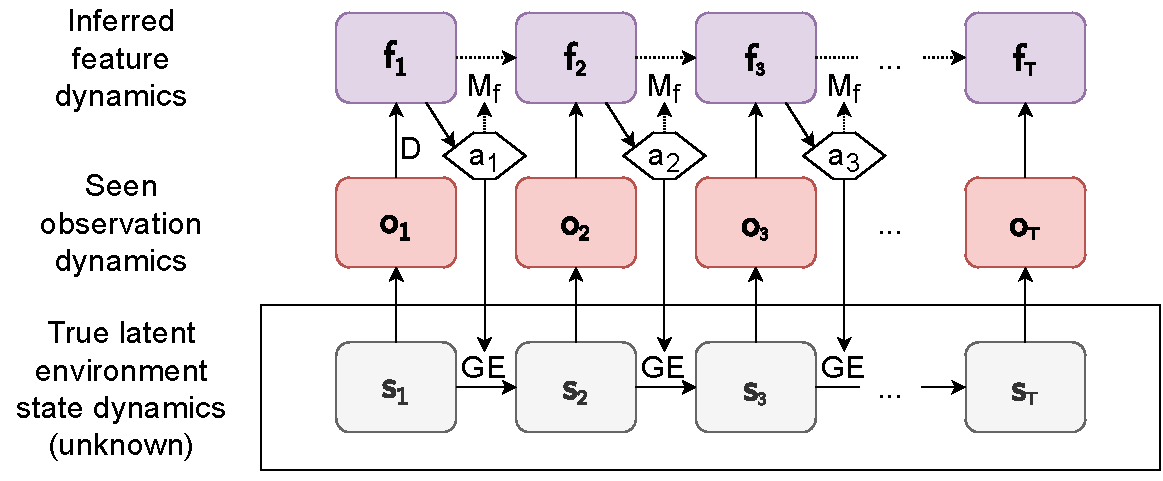
\includegraphics[width=0.7\linewidth]{diagrams/step_spaces}
    \caption{Step representations used in the project. At the bottom, the environment's Game Engine (GE) generates the next state $s_{t+1}$ given the previous state $s_t$ and the action $a_t$. Next, the states are encoded into high-dimensional observations $o_t=E(s_t)$. The true state dynamics $s_t$, as well as the encoder $E$ are unknown. The proposed methods finds a feature space $f_t=D(o_t)$ by applying the decoder $D$. The dynamics in the space of features is modeled by the function $M_f$.}
    \label{fig:step_spaces}
\end{figure}


We have an agent $\pi$ interacting with the environment $\mu$. We start from the model-based Reinforcement learning setup with a decoder and a reconstructor. We would like to obtain the feature space in which the model $M_f$ becomes most simple in terms of a metric $K$. This is the Bayesian approach: with the sparsity prior on the model, we would like to find the posterior distribution over models given the data from the environment.

We consider a model of the environment $\hat{f}_{t+1}=M_f(f_t,a_t)$ in the sense of \autoref{sec:mbrl}. Additionally, we would like some components of $f_t$ and $a_t$ to be ignored when predicting some component of the whole feature vector $f_{i,t+1}$. We view the model $M_f=[M_f^1,...,M_f^f]$ (splitted into scalar functions predicting each feature) as a causal model in the sense of \autoref{sec:causal}. The set of variables of this causal model contains all features, all actions, and additionally the variable $r$ for the reward and the variable $d$ for the "done" (see \autoref{sec:rl} for definitions):
$$
\begin{array}{lcl}
X&=&\{f_1,...,f_f,a_1,...,a_a,r,d\},\\
X_{in}&=&\{f_1,...,f_f,a_1,...,a_a\}\\
X_{out}&=&\{f_1,...,f_f,r,d\}
\end{array}
$$

The variables $X_{in}\subset X$ are the input (ones used for prediction), and the variables $X_{out}\subset X$ are the output (ones being predicted).
We would like to predict the next features, as well as the reward $r$ and the done $d$ at time-step $t+1$ given features and actions at the time-step $t$. The prediction of the model for a variable $x$ consists of pre-multiplying the input features (variables $f_t$ and $a_t$, written as a vector in what follows as $fa_t=[f_t,a_t]\in\mathbb R^{f+a}$) with the binary mask $B_x$, to select the input features, and then applying the SCM function $F_x$: $x_{t+1}=F_x(fa_t\odot B_x)$, $x\in X_{out}$.
$$
\begin{array}{lcllrllr}
\hat{f}_{t+1}^1&=&M_f^1(f_t,a_t)&=&F_{f_1}(&[f_t,a_t]&\odot B_{f_1}&)\\
&...&\\
\hat{f}_{t+1}^f&=&M_f^f(f_t,a_t)&=&F_{f_f}(&[f_t,a_t]&\odot B_{f_f}&)\\
\hat{r}_{t+1}&=&M_f^r(f_t,a_t)&=&F_{r}(&[f_t,a_t]&\odot B_{r}&)\\
\hat{d}_{t+1}&=&M_f^d(f_t,a_t)&=&F_{d}(&[f_t,a_t]&\odot B_{d}&)\\
\end{array}
$$

\section{Measure of complexity}

\subsection{Sparse features are neither necessary nor sufficient for interpretability}
First, we give a detailed example of why feature sparsity does not imply interpretability, and interpretability does not imply feature sparsity.

\begin{example}
    Consider the $2D$ grid-world environment from Figure \ref{fig:env2d2x2} with $H,W>2$. It has $HW$ states. Consider binary features $f_i\in\{0,1\}$. Given the feature dimensionality $f$, we select the first $HW$ most sparse vectors in $\{0,1\}^f$ to map to the states (this is possible in case if $2^f\geq HW$).

    In case if $f=HW$, we have maximal feature sparsity: each feature vector has at most $1$ component. Feature vectors become $1-hot$ vectors coding for the state numbers (except for the $0$ vector). However, the model lacks interpretability because it does not capture the structure of the environment -- it has $2$ independent components $x$ and $y$, and actions affect only the corresponding coordinates.

    One might argue that the feature dimensionality is too high in this case, and this is the cause of the lack of interpretability.

    In case if $HW\approx f+f(f-1)/2$, we use all vectors with $1$ component and all vectors with $2$ components. However, this model is also not interpretable -- it also does not capture the two-dimensional dynamics.

    This shows that feature sparsity in a resonable example is not sufficient for interpretability.

    Now, a coding with two features with $f_1=x$ and $f_2=y$ solves the problem -- each action corresponds to one feature, and features have a simple dynamics.
    However, this coding is not sparse -- in fact, the values of the features are never $0$. This shows that feature sparsity is not necessary for interpretability.
\end{example}

To be fair, sparse features do help interpretability in case if an observation can contain a limited number of objects, one at a time. For example, an observation either contains an enemy, or the health bar. However, these two variables then can be replaced with one and modeled with our framework. We note that our approach also has flaws (see the failure modes below), and the question of defining human "simplicity prior" mathematically in all cases remains open.

In addition, we must clarify the following point. In what follows, we will induce sparsity on the feature vectors, but in a very specific way. First, we consider sparse feature vectors (with some components zeroed out) as an {\em input to the model predicting the same features}, i.e. a dynamics model. The model takes only certain features as the input. Importantly, the sparsity mask is different for predicting different features, and is not reducible to the sparsity of the feature vector as a whole. In fact, for all of the environments that we use, the feature vector is not sparse as a whole.

In contrast, most known interpretable models (natural language inter-sentence dependencies uncovered with attention, causal models used for medical data, physics equations only capturing the neighbours of a particle to describe its dynamic, sparse linear regression) only have few components: they are sparse. In what follows, we will show that some sparse models are not interpretable, and give methods to overcome that.

\subsection{Sparse fan-in models sometimes are sufficient for interpretability, and usually necessary}
We set the proxy for the Kolmogorov complexity for our class of models as the total number of non-zero components in the mask:
$$
\tilde{K}(B)=\sum\limits_{x\in X_{in}}\|B_x\|_0
$$
Note that we only count the complexity of the mask, and do {\em not} count the complexity of the functions $F_x$, or of the decoder $D$. This stems from two reasons. The first reason is purely practical -- there does not exist a measure of complexity for neural networks $F_x$ or $D$ that could be easily optimized for\footnote{One candidate is the norm of the Jacobian as a measure of complexity, however, this norm would be lower for a $\sin(x)$ function than for a linear function $x$ for some arguments, because the derivative is lower. Another option is to use the same technique with disabling features to limit the fan-in of the neurons in the network to induce structural sparsity. However, this would result in an even more non-convex and hard-to-optimize problem than this thesis presents. This approach is out of the scope of this thesis.}. The second reason is there by design. Namely,
This issue is somewhat alleviated by the fact that neural network of fixed architecture can only implement functions of bounded Kolmogorov complexity: it only has a finite number of arithmetic operations. This means that it is important to set the class of functions that represent the decoder $D$ and the model $F_x$ properly. Otherwise, the following situation can occur.

\begin{proposition}{(Too complex decoder)}
    Consider an arbitrary deterministic environment $\mu$ and a deterministic policy $\pi$. With a suitable decoder, it is possible to obtain $\tilde{K}(B)=1$ (minimal value) and $L_{rec}=L_{fit}=0$
\end{proposition}
\begin{proof}
    The main idea is to map a multidimensional space into a single-dimensional one. There are several ways to do that

    \begin{itemize}
    \item Consider the space of all possible states $S=\mathbb R^s$ of the true environment.

    It is possible to bijectively map a unit interval $(0,1)$ to a unit square $(0,1)^2$. The mapping is highly non-smooth, like the Peano curve.
    Using this technique, we map $\mathbb R^s$ to $\mathbb R^{s-1}$. Repeating the process, we eventually map $\mathbb R^s$ to $\mathbb R^1$. Now, there is only a single feature describing the state.

    \item For discrete state spaces, an even simpler approach is possible: since the number of states is finite, it is possible to represent each state using its number. This trick can also work for continuous states with discretization.
    \end{itemize}

    Now, $f=1$ (only $1$ feature is required). Given features $f_t$, we can compute $f_{t+1}$ by first reconstructing the observation (here the bijectivity matters), and then applying the Game Engine:
    $$
    f_{t+1}=D(E(GE(E^{-1}(D^{-1}(f_t))),a_t))
    $$

    Here, the model $M_f$ depends on a single feature (because we only have a single feature), the reconstruction is perfect, and prediction is perfect.

    The complexity $K(B)=3$: the only feature is used to predict itself, as well as the attributes $d$ and $r$.

    While the complexity of the binary mask $B$ is small, the complete model is extremely complex: the functions $D$ and $D^{-1}$ compute the non-smooth bijection mapping a unit interval to a unit square.
\end{proof}

While in practice, it would be hard to find such a function with gradient descent, as it is highly non-convex, there is another example which shows that the complexity of $D$ and $M_f$ should not be exceedingly high:

\begin{figure}[t]
    \centering
    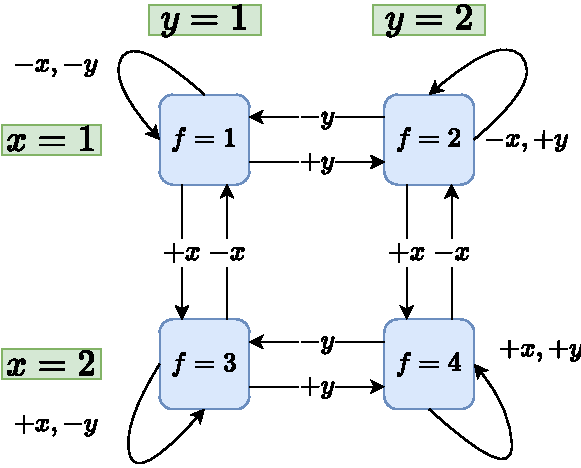
\includegraphics[width=0.7\linewidth]{diagrams/env_2d_2x2.pdf}
    \caption{2D grid-world with 4 cells: 2 rows and 2 columns. Actions $\pm x$ and $\pm y$ change the values of the coordinates. The single feature $f\in\{1,2,3,4\}$ bijectively maps to the state space. This example extends naturally to $H$ rows and $R$ columns with $x\in[H]$ and $y\in [W]$, and the same set of actions $\pm x$, $\pm y$.}
    \label{fig:env2d2x2}
\end{figure}

\begin{example}
    Consider a grid-world with $2$ components of the player: $x$ (horizontal) and $y$ (vertical) taking discrete values: $x\in [H]$ and $y\in [W]$. The actions $-x$ and $+x$ affect the horizontal coordinate $x$. The actions $-y$ and $+y$ affect the vertical coordinate $y$. We can represent this environment by $2$ features, one for each of the coordinates.

    However, consider the case of $H$ and $W$ being small (for example, $H=W=2$). In this case, we can design a transition model using only a single feature $f_1$ which takes the following values:

    $
    \begin{array}{ccc}
        f_1 & x & y \\
        1 & 1 & 1 \\
        2 & 1 & 2 \\
        3 & 2 & 1 \\
        4 & 2 & 2
    \end{array}
    $

    For example, if $x=1$ and $y=2$, we set $f_1=2$.

    Now, the transition model is shown in Figure \ref{fig:env2d2x2}. It is quite complex: each feature variable can potentially result in $3$ different states! However, a neural network with enough layers could fit this dynamics.

    A much simpler model appears if we map each coordinate to a separate feature: $f_1=x$ and $f_2=y$. In this case, the dynamics for each coordinate is much more simple:
    $f_1^{t+1}=\max(1, \min(2, f_1^t+\mathds 1_{a=+x}-\mathds 1_{a=-x}))$

    Thus, too high model complexity will result in less features used, but the interpretability will be lost.

    Luckily, this pathological behavior disappears as $H, W\to\infty$. While the complexity of the coordinate-wise approach does {\em not} become more complex, and is always described as $f_1^{t+1}=\max(1, \min(H, f_1^t+\mathds 1_{a=+x}-\mathds 1_{a=-x}))$, the single-feature approach's complexity increases. First, we show it for the case of "left-to-right" numbering.
    For the single-feature model, we set $f=W\cdot (x - 1)+y$, and we can reconstruct $y=f\mod W$ and $x=(f-y)/W+1$.
    Now, implementing the $z\mod n$ function for $z\in [kn]$ with a neural network of constant complexity is impossible [?????].

    \todo{Seems obvious but very unclear how to prove}

    Therefore, for more states in a dimension ($x$ or $y$), the model would prefer using two features instead of $1$.

    However, this does not prevent at all to learn a linear combination of features: $f_1=\alpha x+(1-\alpha)y$ and $f_2=\beta x+(1-\beta)y$. The dynamics still stays simple.
\end{example}

{\bf "Reusable" decoders and models.} This argument shows a natural setting in which it is not required to count the complexity of the decoder $D$, and of the SCM functions $F_x$. Humans do not re-learn the visual cortex when a new game is presented. Instead, the same architecture is reused, and only the novel high-level behavior is learned. Additionally, humans do not learn the rules of every game from scratch (for example, learning again that there are $x$ and $y$ coordinates in every shooter game). Instead, the existing abstractions (such as $WASD$ keys used to control the player) are re-used. With this in mind, a natural extension of this work is to re-use the decoder and parts of the model (see section \ref{ch:conclusion} for the concrete future direction proposal). If we reuse some parts of the decoder, or of the model, their complexity (in terms of the shortest program describing them) is greatly reduced, when the "bank" of existing abstractions is given, and only an "index" in this "bank" needs to be specified, instead of learning the complete model from scratch.


{\bf Linear models.} A reasonable questions might occur: would it be possible to use the simplest possible class of models to define functions $F$ -- linear models, and "transfer" all of the non-linear complexity into the decoder? This would be extremely beneficial, as environments would be extremely interpretable in this space. The following example shows that even for one of the simplest RL environments, there is no linear feature space that preserves the dynamics and maps bijectively into observations.

\begin{figure}
    \centering
    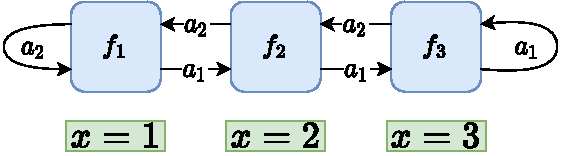
\includegraphics[width=0.7\linewidth]{diagrams/env_line_3}
    \caption{Line environment with 3 states. Action $a_1$ corresponds to moving right, and $a_2$ corresponds to moving left. Going left from the left-most state does not change the sate, and same for the right-most state. The variable $x$ increases when going right and takes integer values starting from $1$. Each state with $x=i$ has an associated feature vector $f_i$}
    \label{fig:env_line3}
\end{figure}


\begin{example}
    Consider the class of linear models: $M_f(f_t,a_t)=M_ff_t+M_aa_t+b$, where $M_f$ is a matrix of size $f\times f$, $M_a$ is a matrix of size $f\times a$, and $b$ is the bias vector of size $f$. We are interested in all environments that can be characterized by linear latent dynamics. In other words, what are all the environments, for which there exist a decoder $D$ and a reconstructor $R$, such that there exist a bijection between the set of observations and the set of feature vectors, and the feature dynamics is linear?

    We show that this class is very small, even with a non-linear decoder. Indeed, consider the Line-3 environment (navigating on a line with 3 states) -- see Figure \ref{fig:env_line3}. It does not fit into our definition.

    Indeed, first, the bias term in the linear model can be shifted into the actions $M_a$. Suppose that the decoder gives some features for the states $f_1, f_2, f_3$ (does not matter how, it's only important that the features are fixed). Multiplying $M_aa_i=A_i$ by definition, this gives two vectors $A_1$ and $A_2$.

    Then, $f_1=M_ff_1+A_2$ (going left from $f_1$ gives $f_1$), and $f_3=M_ff_3+A_1$ (going right from $f_3$ gives $f_3$). Now consider what happens in $f_2$. If we go left, we get $f_1$: $M_ff_2+A_2=f_1$. If we go right, we get $f_3$: $M_ff_2+A_1=f_3$. Subtracting these two gives $f_3-f_1=A_1-A_2$. On the other hand, the "stuck at the wall" equations give us $f_3-f_1=M_ff_3+A_1-M_ff_1-A_2=M_f(f_3-f_1)+A_1-A_2$. So, equating these two, we get
    $f_3-f_1=M_f(f_3-f_1)+A_1-A_2=A_1-A_2$. This means that $M_ff_3=M_ff_1$.

    Now, consider the "stuck at the right wall" $f_3=M_ff_3+A_1$, and going right from $f_1$: $f_2=M_ff_1+A_1$. But $M_ff_1=M_ff_3$, which means that $f_2=M_ff_3+A_1$. Note the same RHS as for the "stuck at the right wall". Therefore, $f_2=f_3$, {\em we cannot distinguish between $f_2$ and $f_3$, degenerate representation.}

    This contradiction shows that for this environment, features are either {\em degenerate} (a single feature vector corresponds to two different observations), or the model should be non-linear.

    Note that a simple non-linear model is applicable for this environment:
    $f_1=x$, $f_1^{t+1}=\min(3, \max(1, f_1^t+\mathds 1_{a=a_1}-\mathds 1_{a=a_2}))$.
\end{example}

These examples show that it is important to set the complexity of the model's neural networks correctly. A too simple model would never fit the environment, and a too complex model can give non-interpretable features.

A practical way to choose the measure of complexity is to first fit a model without sparsity constraints, select one with minimal complexity still fitting the data, and then run \sysname.

\section{Optimization problem for \sysname}
\begin{figure}[h]
    \centering
    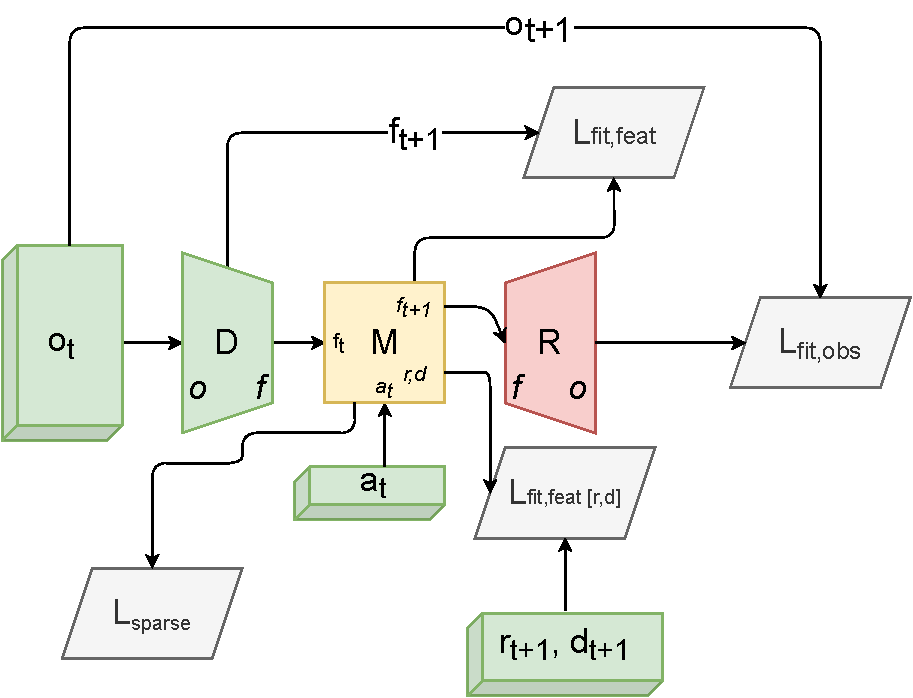
\includegraphics[width=0.7\linewidth]{diagrams/architecture_losses}
    \caption{The diagram of losses for \sysname. The batch of observations $o_t$ (left) is fed into the {\em decoder} $D$, which outputs {\em features} $f_t$. The next features $f_{t+1}$ are predicted using the model $M$ given the actions $a_t$. The model is regularized with a sparsity constraint $L_{sparse}$, and fit using losses $L_{fit,feat}$ in the feature space (predicting the next features) and in the observation space (predicting the next observation). The model also predicts the additional reward (r) and done (d) features. The reconstruction loss is not shown on this figure. See this section for more details on the losses.}
    \label{fig:architecture_losses}
\end{figure}


Overall, we would like to obtain a sparse model without loss of fit quality. Our search space consists of continuous parameters for $D,R,F_x$, and discrete parameters $B_x$ for $x\in X_{in}$ (see above). The figure \ref{fig:architecture_losses} shows the trainables and the losses described in this section.

\subsection{Relative mean-squared error loss}
In order to know how well the model predicts the next state, we use a {\em relative} mean-squared error loss, instead of the standard "absolute" one. Specifically, if the model predicts $\hat{y}_t$, for $t\in[T]$, and the true values are $y_t$, $t\in[T]$, the relative MSE error is defined as:
\begin{equation}
\label{eq:rel_mse}
\rho(y_t, \hat{y}_t|t\in[T])=\frac{1}{T}\sum\limits_{t=1}^T\left(\frac{y_t-\hat{y}_t}{\sigma[y]}\right)^2
\end{equation}
Here, $\sigma[y]$ is defined as standard deviation of $y$ in case if it is non-zero, and it is defined as $1$ otherwise.

\begin{example}
    Suppose that $T=2$, $y_{\cdot}=\varepsilon\cdot (0,1)$ and $\hat{y}_{\cdot}=\varepsilon\cdot (1, 0)$. We compute $\sigma[y]=0.5\varepsilon$, and $\rho(y_t,\hat{y}_t)=4$. This value does not depend on the scale $\varepsilon$ of $y$ and $\hat{y}$. In contrast, the traditional mean-squared error would yield $\rho_{mse}(y_t,\hat{y}_t)=\frac{1}{T}\sum\limits_{t=1}^T\left(y_t-\hat{y}_t\right)^2=0.5\varepsilon^2(1^2+1^2)=\varepsilon^2$, which depends on the scale of the features.

    It is important that the quality metric does not depend on the magnitude of the inputs, as the magnitude of the predicted features can be arbitrary high or low.
\end{example}

\begin{example}
    Suppose that $y\sim Y$ (i.i.d. samples from a distribution $Y$), and $\hat{y}=c$ is a constant predictor. Then, the best value of the relative MSE loss $\rho$ is $1$ with $c=\mathbb EY$. Since neural networks can fit a constant, we expect that $\rho<1$ in our experiments. However, at the beginning of the training, this value can be larger than $1$.
\end{example}

\begin{example}{(Discrete-valued variables)}
    Suppose that $y\sim Uniform([n])$ -- a discrete uniform variable taking values in $\{1,...,n\}$. $\mathbb Ey=n/2$ and $\var y=(n^2-1)/12$. In case if $\rho(y,\hat{y})<\varepsilon<\frac{1}{2n}$, we compute using the Chebyshev's inequality: $p_{bad}=P(y\neq \hat{y})=P(|y-\hat{y}|>1)\leq \mathbb E(y-\hat{y})^2/1^2=O(\rho n^2/12)$. If we want $p_{bad}=1/n$, we obtain a requirement $\rho<12/n^3$. For a discrete variable with $n=20$ to obtain $p_{bad}<1/20$, we will have to have $\rho\approx1.5\times 10^{-3}$.

    However, if we specify $|y-\hat{y}|\sim Uniform([0, a])$, we have $\var |y-\hat{y}|=(a^2)/12$, and the condition $P(|y-\hat{y}|>1)\leq 1-1/a$. Setting $P(|y-\hat{y}|>1)<1/n$ gives $a<n/(n-1)$. Since $\rho=O(a^2/n^2)$, we arrive at a looser condition $\rho< 1/n^2$. For example, for a discrete variable with $n=20$, to obtain $p_{bad}<1/20$, we will have to have $\rho\approx 3\times 10^{-2}$.
\end{example}

\begin{example}
    Suppose that $y=0$ (a constant), and $\hat{y}\sim N(0, \sigma^2)$ -- the normal distribution. In this case, $\sigma[y]=1$ (because the true variance is $0$), and $\rho(y, \hat{y})=\mathbb E_{\hat{y}\sim N(0, \sigma^2)}(0-\hat{y})^2=\sigma^2$.
\end{example}

\begin{example}
    Suppose that $y\sim N(0, \sigma^2)$ (normal distribution), and $\hat{y}=0$ -- a constant. In this case, $\sigma[y]=\sigma$ and $\rho(y, \hat{y})= 1/\sigma^2 \mathbb E_{y\sim N(0, \sigma^2)}(y-0)^2=\sigma^2/\sigma^2=1$.
\end{example}

\subsection{Degenerate decoder}
The decoder needs to be invertible (or, at least, "partially" invertible). Note that, technically, it is possible for the decoder to always output $0$ for all observations. In this case, there exist a simple constant model that "predicts" the next state perfectly (if prediction for $d$ and $r$ is disabled). However, such a model is useless, as it does not describe any aspect of the dynamics. One way to solve this issue is to introduce a reconstructor predicting observations from features. See \autoref{sec:mbrl} for further discussion.

The reconstruction loss is defined in terms of the expected distance between the reconstructed and true observations:
\begin{equation}
\label{eq:reconstruction_loss}
L_{rec}=\mathbb E_{h\sim (\mu\leftrightarrow \pi)}\rho(R(D(o_t)), o_t|t\in [T])
\end{equation}

\subsection{Model fit in observation and feature space}
We also would like the model to predict the future time-steps correctly. This can be achieved in one of two ways.

\begin{enumerate}
    \item Feature-space loss. We penalize the models' features if they deviate from the features predicted by the decoder at the next time-step:
    \begin{equation}
    \label{eq:loss_fit_feature}
    L_{fit,feat}=\mathbb E_{h\sim (\mu\leftrightarrow\pi)|T>1}\rho(M_f(D(o_t), a_t), D(o_{t+1})|t\in [T-1])
    \end{equation}

    Here, we only consider episodes that last more than $1$ time-step, because otherwise there is no "next" time-step to predict.\footnote{We do not model the "initial state" distribution, because it does not affect model simplicity in terms of $K(B)$, and it does not affect the SCM functions $F_x$, and in this project we are only interested in learning the causal graph.}

    \item Observation space loss. We penalize the model if the {\em reconstructed observation} given the predicted features matches the true next observation:

    \begin{equation}
    \label{eq:loss_fit_obs_space}
    L_{fit,obs}=\mathbb E_{h\sim (\mu\leftrightarrow \pi)|T>1}\rho(R(M_f(D(o_t), a_t)), o_{t+1}|t\in [T-1])
    \end{equation}
\end{enumerate}

Next, we compare the two approaches. First, if $L_{fit, feat}=0$, it follows that $L_{fit, obs}=0$. Indeed, the reconstruction loss $L_{rec}$ ensures that the next-step features result in correct observations. And $L_{fit, feat}=0$ ensures that the features are predicted correctly.

In contrast, $L_{fit,obs}=0$ does {\em not} imply that $L_{fit, feat}=0$. Indeed, the model can add the $1$-st feature to all features: $\hat{f}_i=f_i+f_1$ and indicate that by adding a large enough number to another feature: $\hat{f}_s=f_s+10\sigma[f_s]$. The decoder first determines if $10\sigma[f_s]$ was added to $f_s$, and then either subtracts $f_1$ or keeps it. This way, $L_{fit, feat}=0$, but the model does not predict the correct features. This mean that in practice, we need to use $L_{fit,feat}$, and, otherwise, the learned model function does actually predict the next features, and, thus, the causal graph might be incorrect.

\begin{example}{(Incorrect causal graph when only using $L_{fit, obs}$)}
    Consider the Game Engine from Figure \ref{fig:env2d2x2}. The features predicted by the decoder are $x$ and $y$ (not the ones in the figure).
    The model is the following function: $\hat{x}_{t+1}=x_t+10\cdot\mathds 1_{a=+y}-10\cdot\mathds 1_{a=-y}$, $\hat{y}_{t+1}=y_t+10\cdot\mathds 1_{a=+x}-10\cdot\mathds 1_{a=-x}$.
    It is possible to obtain $L_{fit, obs}=0$, because we can reconstruct both the previous state, and the action from $\hat{x}$, $\hat{y}$. Indeed, note that $|x_t|,|y_t|<2$. This means that, if $\hat{x}>10$, an action $+y$ was taken. The rest of the actions are reconstructed in the same way.
    Next, knowing the actions we obtain $x_t$ and $y_t$. Next, the reconstructor performs "the function of the model", computes the (true) next $x_{t+1}$ and $y_{t+1}$, and then performs the reconstruction.
    In case if both of input arguments to the reconstructor are $|x_t|<10$ and $|y_t|<10$, the model does not perform the time-step prediction.

    The causal graph in this case is incorrect: $x$ depends on $+y$ and $-y$, and $y$ depends on $+x$ and $-x$.
\end{example}

Therefore, we have to use $L_{fit,feat}$. However, in practice, even when using the relative loss, $L_{fit, feat}<\varepsilon$ for a small $\varepsilon\in(0,1)$ does {\em not} mean that the prediction quality is good.

\begin{example}
Consider the Game Engine from Figure \ref{fig:env2d2x2}. It has $2$ latent variables: $x$ and $y$. Now, suppose that the features (not on the figure) are $f_1=x$ and $f_2=\alpha y+(1-\alpha)x$ for $\alpha \ll 1$. Suppose that $L_{fit, feat}<\varepsilon$. Does it mean that the model "preserves" the information both about $x$ and $y$? No.

Indeed, for the variable $x$, $L_{fit, feat}<\varepsilon$ implies that $\rho(x,\hat{x})<\varepsilon$, as required. However, for $y$, it does not. Indeed, we can show that it is possible to obtain any $\varepsilon$ bound on th e loss given $\hat{y}=\mathbb y$ (the constant prediction giving $\rho(y,\hat{y})=1$. Assume that $x$ is predicted perfectly. Next, consider

$$\rho(\alpha y+(1-\alpha)x,\alpha \hat{y}+(1-\alpha)\hat{x})=\frac{\mathbb E \left(\alpha(y-\hat{y})+(1-\alpha)(x-\hat{x})\right)^2}{\sigma[\alpha y+(1-\alpha)x]^2}$$.

We assume that $x$ and $y$ are independent under $\pi$ and have the same variance of $c$. Then we compute $\sigma[\alpha y+(1-\alpha)x]^2=\sqrt{\alpha^2+(1-\alpha)^2}c$.

Next, since $\hat{x}=x$, $\rho=1/\sigma^2\alpha^2\mathbb E(y-\hat{y})^2=\frac{\alpha^2}{\alpha^2+(1-\alpha)^2}$. Since this equation has a limit of $0$ when $\alpha\to 0$, and since the decoder is free to set $\alpha$ arbitrarily small, we can make $L_{fit, feat}$ arbitrarily small, while the model only predicts the value of $x$, but not the value of $y$.

Note that, without the relative loss, it is not even required for the model to predict the value of $x$. Indeed, to make the loss arbitrary small, it is sufficient for the decoder to reduce the magnitude of the features, and for the reconstructor to increase the input weights.
\end{example}

Therefore, we have to use both losses, one in the feature space, and one in the observation space.

\subsection{Sparsity loss}
In \autoref{sec:grad_discrete} we outline techniques for parameterizing $B\sim Be(P)$ and then computing the gradient $\partial B/\partial P$, so it becomes possible to find the values of $B$ using gradient descent.

Now we consider the original objective:
$$
K(B)=\sum\limits_{x\in X_{in}}\|B_x\|_0
$$

Since $B$ is sampled from a distribution $P$, we compute the expected value:
$$
\mathbb E_{B\sim Be(P)}K(B)=\sum\limits_{x\in X_{in}}\|P_x\|_1
$$.

This happens because for each component, $\mathbb E_{b\sim Be(p)}b=p$. Thus, we naturally arrive at the $l_1$-relaxation of our discrete problem [cite Bengio].

We define this loss as:
$$
L_{sparse}=\mathbb E K(B)=\sum\limits_{x\in X_{in}}\|P_x\|_1
$$

\subsection{Ranges of probabilities and exploration}
In case if for some of the probabilities $P_{xx'}=0$, or $P_{xx'}=1$, that feature is {\em never} selected and is never active, or is {\em always} selected, and the model never explores cases where this feature is not enabled.

However, we would like to have the case $P_{xx'}=1$ possible in our system. Indeed the difference in losses $L_{fit}\big|_{B_{xx'}=0}$ and $L_{fit}\big|_{B_{xx'}=1}$ can be drastic, and in the worst case we have $L_{fit}\big|_{B_{xx'}=0}-L_{fit}\big|_{B_{xx'}=1}=f+2$ (without using the important feature, each output feature can only be predicted as a constant, and the same for reward and done). Therefore, if $p_{\max}<1$, we have $L_{fit}=(f+2)(1-p_{\max})$, and the loss will no go lower than this value.

Another issue that $p_{\max}<1$ yields is duplicated features. Indeed, if an important feature is only given with probability $p_{\max}<1$ and $\varepsilon=1-p_{\max}$, it would be beneficial to decrease the loss $L_{fit}$ to duplicate this feature (the decoder uses a spare feature to output the same value). Then, the model would {\em not} receive the value for an important feature with probability $\varepsilon^2$, instead of $\varepsilon$. This decreases the loss $\varepsilon$ times. Therefore, training the model with $p_{\max}<1$ would likely lead to feature duplication.

In contrast, $p=p_{\min}>0$ would not have significant effects on the loss, as adding a non-important feature cannot improve the loss significantly, and definitely cannot worsen the loss (because more features are used). Now, since $p=p_{\min}\approx 0$, we have
$$
L_{fit}=p\underbrace{L_{fit}\big|_{B_{xx'}=1}}_{L_1}+(1-p)\underbrace{\L_{fit}\big|_{B_{xx'}=0}}_{L_0}
$$
Since $L_1\leq L_0$, $L_{fit}\leq pL_0+(1-p)L_0=L_0$, and $L_0\geq L_{fit}$. On the other hand, $L_{fit}\geq (1-p)L_0$, which gives $L_0\leq \frac{L_{fit}}{1-p}= L_{fit}(1+p+O(p^2))\approx L_{fit}(1+p)$.

This means that $L_0\in (1, 1/(1-p))L_{fit}$. For $p=p_{\min}\approx 0$, the gap between the two solutions is small: $L_0\approx L_{fit}$.

It means that the loss with $B_{xx'}$ disabled is upper-bounded by the current loss $L_{fit}$ (where $B_{xx'}$ is only enabled with a small probability). To output the final answer causal graph, we could threshold these probabilities to $0$, and the answer would only worsen a small amount in terms of the fit quality.

\begin{example}
    Let's consider different cases, assuming that the model was fitted to convergence on a set of features with a fixed tensor of probabilities. Consider the case of $2$ input and output features, with features being equal and having a deterministic relationship (from input to output).
    \begin{enumerate}
        \item $p=0$ for all pairs. In this case, no features are given to the model, and the model will learn to predict the mean of the output features. The causal graph is empty. The loss is equal to $2$ (since standard deviation for each feature is $1$ w.l.o.g. because of the relative error).
        \item $p=1$ for all pairs. In this case, the model uses all features, and the error is minimal. The loss is $0$.
        \item $p=0.5$ for all pairs. In this case, the model will try to extract as much information as possible when the feature is present. Essentially, with probability $0.25$, the model will give the mean output feature, and with probability $0.75$ it will use either one of the input features, or both of them. The loss is equal to $2\times 0.25=0.5$.
        \item In the general case $p\in [0, 1]$, the model has an error of $2$ with probability $(1-p)^2$ and a loss of $0$ with probability $1-(1-p)^2$. The expectation is $2(1-p)^2$.
    \end{enumerate}

    Now consider a similar case when the mutual information between features is $0$ (they are independent). In this case, for a probability $p$, we have the loss being $2$ with probability $(1-p)^2$, a loss of $1$ with probability $2p(1-p)$ and a loss of $0$ with probability $p^2$. The expectation is $2(1-p)^2+2p(1-p)=2-4p+2p=2-2p=2(1-p)$. This loss is higher than for the case of equal features for all $p\in (0,1)$.

    To avoid a case when there are no samples with $\xi=1$ (with low $p$), we limit the range of $p$ to be $p\geq p_{\min}=0.01=1\%$. Setting this value higher results in feature duplicates, as the model tries to predict the outputs even from partially present features. A value of $1\%$ with a batch size of $T=5000$ gives $50$ samples with $\xi=1$ in the worse case (on average), which is empirically sufficient to turn features on. To turn the features off, we introduce a sparsity regularizer.
\end{example}

\subsection{Non-stationarity and adding the mask to the model}
Consider the data that the functions $F_x$ are fit on, when the probabilities $P$ change:
$$
fa_t\odot B_x\to x_{t+1}
$$

Since $B_x$ depends on $P_x$, the dataset clearly depends on $P$. Since the probabilities change during the training (a feature could be turned on and off repeatedly in search of the best graph), the problem becomes highly non-stationary -- effectively, the model has to re-relearn to rely on the new set of features that it did not see before. In addition, in case of discrete features, the model might not be able to distinguish between the case where $fa_t=0$ or $B_x=0$.
It may happen that in case if $f_1=0$ is given, the model should rely on $f_1=0$. However, if a feature is not given, the model should rely on another, more noisy feature.
However, an input of $0$ does not allow to distinguish between these cases, and the model would be forced to "guess" (output the expected value between the two datasets).
A solution for this is to feed the mask to the model as well:
$$
\hat{x}=F_x(fa_t\odot B_x,B_x)
$$

\subsection{Separate exploration loss}
To speed up the convergence even more for the cases $p\approx 0$ and $p\approx 1$, we temporarily threshold the probabilities to be in the range $[p^{expl}_{\min},p^{expl}_{\max}]$, and fit the models with masks $B$ sampled from this distribution. This results in the loss
\begin{equation}
L_{fit}\big|_{p:=p^{expl}}=\mathbb E_{B\sim Be(p^{expl})} L_{fit}
\end{equation}

\subsection{Additional feature transformation ("rotation")}
\begin{figure}[h]
    \centering
    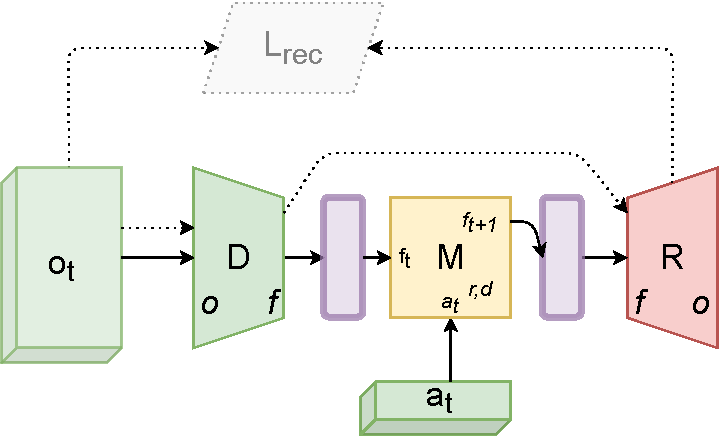
\includegraphics[width=0.7\linewidth]{diagrams/architecture_rotation}
    \caption{Two additional linear feature transformations (purple) applied before and after the model $M$ in order to speed up the convergence. The reconstruction loss path (dotted) bypasses the additional transformations. See \autoref{fig:architecture_losses} for the full description of the components}
    \label{fig:architecture_rotation}
\end{figure}


During training, the distribution for the decoder is non-stationary, because the feature space changes to optimize for sparsity. This happens because the model affects the decoder, and the reconstructor must match the decoder. In order to alleviate this issue, two separate linear transforms are added right before and after the model (see Figure \ref{fig:architecture_rotation}). These transforms allow to quickly enable or disable features, or to change the linear combination of them:
$$
\begin{array}{clll}
L_{fit, obs}&=\rho(R(Z_{post}(M_f(Z_{pre}(D(o_t)),a_t))), o_{t+1});& R\circ Z_{post}\circ M_f \circ Z_{pre}\circ D&\mapsto o_{t+1},\\
L_{fit, feat}&=\rho(Z_{post}(M_f(Z_{pre}(D(o_t)),a_t)), D(o_{t+1}));&Z_{post}\circ M_f\circ Z_{pre}\circ D&\mapsto Do_{t+1},\\
L_{fit, m-feat}&=\rho(M_f(Z_{pre}(D(o_t)),a_t), Z_{pre}(D(o_{t+1})));&M_f\circ Z_{pre}\circ D&\mapsto Z_{pre}\circ Do_{t+1}.\\
\end{array}
$$

\subsection{NP-hardness in the general case}
As in the linear case of the semester project, we prove the NP-hardness of finding the most sparse causal graph that fits the data. While it was shown [?] that finding the causal graph without a decoder is not NP-hard, it is if we consider a learned representation as well

\todo{reduction to sparse dictionary learning}

\subsection{Optimization schemes}
Now, we have a number of losses (see Figure \ref{fig:architecture_losses} for a diagram of all components) that we would like to minimize together

\begin{equation}
\label{eq:all_losses}
\begin{array}{lc}
L_{sparse}&\to\min\limits_P\\
L_{rec}&\to\min\limits_{D,R}\\
L_{fit, feat}&\to\min\limits_{D,M,P,R}\\
L_{fit, obs}&\to\min\limits_{D,M,P,R}
\end{array}
\end{equation}

Ideally, we would like to find a point which jointly minimizes all of these losses. In the case of a deterministic environment, it is possible to achieve all of the losses being $0$, $L_{sparse}$ having the minimal possible discrete value.

The traditional practical reformulation of this problem in terms of a Machine Learning problem would result in a loss consisting of two components: one to fit the parameters of the posterior to the data, and one to regularize the model for sparsity, with a coefficient $\lambda$ controlling how "strong" is the posterior.
Such an approach, however, requires to "guess" the parameter $\lambda$.
A much more convenient way is to either guess the target number of edges in the graph $K(B)$, or the losses constraint $L_i\leq c_i$ for $i\in\{fitobs, fitfeat, rec\}$.
We present the approaches below:


\begin{itemize}
    \item Linear combination of losses with constant coefficients:

    \begin{equation}
    \label{eq:opt_scheme_linear_comb}
    \mathcal L=\lambda_{sparse}\cdot L_{sparse}+\lambda_{fit,feat}\cdot L_{fit, feat}+\lambda_{fit,obs}\cdot L_{fit, obs}+\lambda_{rec}\cdot L_{rec}\to\min\limits_{D,M,R,P}
    \end{equation}

    \item Constrained problem with sparsity guess:
    \begin{equation}
    \label{eq:opt_scheme_sparsity_guess}
    \begin{array}{ll}
    \min\limits_{D,M,R,P}& \lambda_{fit,feat}\cdot L_{fit, feat}+\lambda_{fit,obs}\cdot L_{fit, obs}+\lambda_{rec}\cdot L_{rec}\\
    s.t.& L_{sparse}\leq c_{sparse}
    \end{array}
    \end{equation}

    \item Constrained problem with fit guess and a linear combination:
    \begin{equation}
    \label{eq:opt_scheme_fit_guess_lin_comb}
    \begin{array}{ll}
    \min\limits_{D,M,R,P}& L_{sparse}\\
    s.t.&\lambda_{fit,feat}\cdot L_{fit, feat}+\lambda_{fit,obs}\cdot L_{fit, obs}+\lambda_{rec}\cdot L_{rec} \leq c_{fit, comb}
    \end{array}
    \end{equation}

    \item Constrained problem with granular fit guess:
    \begin{equation}
    \label{eq:opt_scheme_fit_guess_granular}
    \begin{array}{ll}
    \min\limits_{D,M,R,P}& L_{sparse}\\
    s.t.&L_{fit, feat}\leq c_{fit, feat}\\
    s.t.&L_{fit, obs}\leq c_{fit, obs}\\
    s.t.&L_{rec}\leq c_{rec}
    \end{array}
    \end{equation}
\end{itemize}

We compare the versions \ref{eq:opt_scheme_linear_comb}, \ref{eq:opt_scheme_sparsity_guess}, \ref{eq:opt_scheme_fit_guess_lin_comb}, \ref{eq:opt_scheme_fit_guess_granular} in \autoref{ch:evaluation}.

In terms of the ease of use, \autoref{eq:opt_scheme_fit_guess_granular} requires least knowledge about the problem. Indeed, we only set the relative thresholds for the losses (values less than $1$), and obtain the most sparse causal graph allowing for such a loss.

{\bf Solving constrained problems.} To solve the constrained problems with gradient descent we use the Lagrange primal-dual method. We consider the Lagrange function for the \autoref{eq:opt_scheme_fit_guess_granular}:
$$
L_{agrange}=L_{sparse}+\lambda_{fit, feat}(L_{fit, feat}-c_{fit, feat})+\lambda_{fit, obs}(L_{fit, obs}-c_{fit, obs})+\lambda_{rec}(L_{rec}-c_{rec})
$$

We note that solving \autoref{eq:opt_scheme_fit_guess_granular} corresponds to solving
\begin{equation}
\label{eq:opt_lagrange}
\min\limits_{D,M,R,P}\max\limits_{\{\lambda_i\geq 0\}}L_{agrange},\,i\in\{fitfeat, fitobs, rec\}
\end{equation}

Indeed, an an optimal point of \autoref{eq:opt_scheme_fit_guess_granular} is a saddle point of \autoref{eq:opt_lagrange} [known fact]. Roughly speaking, this happens because if a constraint is violated, any $\lambda>0$ results in an infinite value of the loss.

To solve this problem, a primal-dual descent-ascent method can be applied (here $x=(D,M,R,P)$ -- the parameters of all neural networks):

\begin{equation}
\label{eq:primaldual}
\begin{array}{rl}
x_{t+1}&=x-\eta\frac{\partial L_{agrange}}{\partial x}\\
\lambda_i&=\lambda_i+\eta\frac{\partial L_{agrange}}{\partial \lambda_i},\,i\in\{fitfeat,fitobs,rec\}
\end{array}
\end{equation}

For convex functions, this algorithm is known to converge to a saddle point of \autoref{eq:opt_lagrange}. The algorithm has the following intuitive interpretation. Suppose that $\lambda_i$ is small, and $i'th$ constraint is violated: $L_i>c_i$. Since $\frac{\partial L_{agrange}}{\partial \lambda_i}=L_i-c_i>0$, the parameter $\lambda_i$ would increase. If, in contrast, the constraint has a slack (is not violated) and $L_i<c_i$, the parameter $\lambda_i$ would decrease to allow optimizing for the objective $L_{sparse}$.
Therefore, we expect the following dynamics: first, the algorithm would turn most of the features on in order to satisfy the constraints, and then it would optimize for sparsity.

If we apply this algorithm for the other (symmetric) formulation of our problem (\autoref{eq:opt_scheme_sparsity_guess}), it would first disable features, and then, once the target sparsity level was reached, it would care about fitting the reconstructor and the SCM functions.

%{\bf Sparsity has to be lower than required sometimes.}

Introduce and discuss the design decisions that you made during this project.
Highlight why individual decisions are important and/or necessary. Discuss
how the design fits together.

This section is usually 5-10 pages.


%%%%%%%%%%%%%%%%%%%%%%%%
\chapter{Implementation}
\label{ch:implementation}
%%%%%%%%%%%%%%%%%%%%%%%%
In this chapter we discuss the specific of our implementation of \sysname. We touch such issues as the initialization of the probability metrics, tips and know-how during training, and the project structure.

\subsection{Initialization}
We initialize the probability matrix to be an identity for the features (a feature only affects itself), and to a full matrix for the rest (actions, reward and done). We this method to initializing with all zeros, all ones, or a random initialization in the next section

\subsection{Metrics}
In order to assess the quality of the solution, we track the following quantities:
\begin{itemize}
    \item Sparsity gap. We compute $L_{fit}$ with the current mask $B\sim Be(P)$, as well as with a fully-enabled mask (or the complete causal graph) $B_{xx'}=1$. This gives losses $L_p=L_{fit}^{p}$ and $L_{full}=L_{fit}^{p:=1}$.

    Now, we define $\Delta^{add}_{sparse}=L_p-L_{full}$. This quantity is positive if the model is fit well (adding features should not worsen the prediction quality). The value of this metric shows how well feature selection has worked: if the value is high, it means that some of the required for prediction features are currently disabled (or, that the model is not fit enough).

    A multiplicative version $\Delta^{mult}_{sparse}=\frac{L_p-L_{full}}{L_p}$. This value is positive when $\Delta^{add}$ is positive, and this value is less than $1$, because $L_{full}>0$

    \item Number of edges in the graph, or the number of large components in the matrix $P$. We compute a k-means clustering\footnote{A simple thresholding with $p=0.5$ would suffice to obtain the final graph, however, the benefit of K-means is that it works even when the training is not fully complete, and the probabilities are not fully $p_{\min}$ or $1$. This allows the see manually the preliminary results while training and quickly understand if the trial is likely to be successful.} in 1-dimensional space of all probabilities $\{P_{xx'}\}_{x\in X_{in},x'\in X_{out}}$. This gives a threshold $\tau\in[0,1]$. Next, we select the pairs $(x, x')$ such that $P_{xx'}>\tau$. This gives the answer causal graph, and the number of non-zero components.

    \item Total entropy of distributions $Be(P_{xx'})$. This quantity should be low at the end of training, because all features should be either turned on or off.
\end{itemize}

\subsection{Separate networks to predict pixels and models}
Since we would like our features to be disentangled (corresponding to different things), there is (by definition) no benefit of multi-task learning. In our experiments (see \autoref{ch:evaluation}) we show that multi-task learning harms convergence speed in case if the tasks are not related. We explain it by the fact that a shared model has layers that are used by all tasks. If the tasks are not related, it is hard for gradient descent to "split" the neurons between tasks, as all of them "want" to use the neurons at a layer. The same applies to the reconstructor (predicting weakly correlated pixels in a toy grid world), and the decoder (predicting features that are disentangled)\footnote{In case of a convolutional decoder, this part is shared, but the subsequent fully-connected layers are not. Decoding the image is a shared task, but decoding features from that representation is not}.

In order to implement the separate networks we use the {\tt einsum} operator in pytorch to implement "vectorized" fully-connected networks.

\subsection{Project code structure}
The code can be found in our \href{Github repository}{https://github.com/sergeivolodin/causality-disentanglement-rl}. The code uses gin config files for modular configuration, ray tune for hyperparameter tuning, Tensorboard for tracking metrics real-time, and Sacred to save all the data from all experiments.

\subsection{Data collection and the true distribution}
We run $k$ parallel data collection processes with ray, and aggregate the data in one ring buffer process. Each minibatch is sampled as random steps from all of the collected episodes and given to the learner class. The ring buffer process maintains the ratio of collected steps to sampled steps to be at least a constant fraction $\zeta=0.5$ to prevent overfitting to only collected steps.

We note that this does not result in a true distribution $\mathbb E_{h\sim (\mu\leftrightarrow\pi)}\mathbb E_{t\sim Uniform([T])}$. The true distribution requires us to sample one episode, select a random step, and then discard the rest of the episode. Effectively, it would require to set $\zeta=\mathbb E_{h}T$: we sample $T$ times more steps than "required". This would slow down the convergence significantly. In a minibatch from the true distribution, all the steps are likely to be from different episodes. This is important for procedurally-generated environments which have a different layout for each new episode.

\subsection{Number of optimizers}
Consider the loss from \autoref{eq:opt_scheme_linear_comb}. It depends on multiple groups of variables: the decoder $D$, the model $M$, the reconstructor $R$, and the matrix of probabilities $P$. We test two options for optimizing $L$:
\begin{itemize}
    \item One optimizer, updating each group of variables at every iteration.
    \item $4$ optimizers, each updating one of $\{D,M,R,P\}$, and doing multiple steps at a time. This corresponds to finding the optimum a bit more precisely for one group of parameters. The rationale is the following. Since for a single group of parameters (such as $M$), the problem looks more like supervised learning (the model receives a stationary distribution of inputs, and has to fit a stationary distribution of outputs), the problem becomes more like what neural networks are well-tested at -- supervised learning, albeit only for a few iterations.
\end{itemize}

\subsection{Time-scale separation for Lagrange multipliers}
Sometimes the order of magnitude of $\lambda_i$ in \autoref{eq:opt_scheme_fit_guess_granular} or \autoref{eq:opt_scheme_fit_guess_lin_comb} needs to be changed significantly. For example, the value of the sparsity has recently decreased significantly, which leads to a much bigger emphasis on the constraints. We need to decrease the Lagrange multiplier, or, otherwise, too little emphasis is put on decreasing sparsity even more. With standard parameterization, $\lambda_i$ would decrease exponentially like in standard Gradient Descent.

If we reparameterize $\lambda_i=\sqrt{\mu_i}$, or $\lambda_i=\mu_i^2$ or $\lambda_i=\exp(\mu_i)$, the parameter $\lambda_i$ would change slower (in the first two cases) or faster (in the last two cases). Such a difference cannot be achieved by simply changing the learning rate for $\lambda_i$, as such modifications would only change the "slope of the line", while reparametrization changes the asymptotic behavior (for example, a line vs. a quadratic function).

A result shows that a sufficient time-scale separation is crucial [GAN learning rate paper].

custom gradient for gumbel, custom exponential "annealing"

selecting coefficients

The implementation covers some of the implementation details of your project.
This is not intended to be a low level description of every line of code that
you wrote but covers the implementation aspects of the projects.

This section is usually 3-5 pages.


%%%%%%%%%%%%%%%%%%%%
\chapter{Evaluation}
\label{ch:evaluation}
%%%%%%%%%%%%%%%%%%%%
In this section, we present the results of running \sysname on a number of benchmark environment that we develop, as well as on established baselines.
We denote the resulting graph given by the algorithm as $\hat{G}_{x'x}$ for whether there is an edge from a cause variable (one at the current time-step) $x\in X_{in}=\{f_1,...,f_f,a_1,...,a_a\}$ to an effect variable (one at the next time-step) $x'\in X_{out}=\{f_1,...,f_f,r,d\}$ (see \autoref{ch:design}). The true causal graph for an environment (if exists) is denoted as $G_{x'x}$. The matrices $G_{x'x}$ and $\hat{G}_{x'x}$ have binary values $G_{x'x}\in\{0,1\}$. $1$ means that the edge is present, and $0$ means that the edge is absent. The total number of edges is $K(G)=\sum\limits_{x\in X_{in}}\sum\limits_{x'\in X_{out}}G_{x'x}$. To obtain $\hat{G}$ from $P$, a thresholding algorithm (K-Means) is applied (see \autoref{ch:implementation} and \autoref{ch:design}).

\section{Environments}
We describe the environments that we develop for this project, as well as established benchmarks.

\subsection{SparseMatrix$(n,k)$ environment}
The simplest environment we consider is SparseMatrix(n,k). Given the dimensionality of the space, we randomly sample a matrix $A\in \mathbb R^{n\times n}$ at the initialization of the environment (once per training session, i.e. the matrix is the same after a {\tt reset()}).

The matrix $A$ is sampled to have $k\geq n$ non-zero component and that it is non-degenerate. We first permute the numbers $[n]$, and then set $A_{ij}:=\pm 1$.
After that, elements $k-n$ are added to random "free" (zero) spots $A_{ij}:=\pm 1$.

At each episode, the state of the environment is initialized as $s_1^i\sim N(0,1)$ for $i\in[n]$. At each time-step, the state is multiplied by the transition matrix:
$$
s_{t+1}=As_t
$$

The actions are ignored for this environment, and the reward is always $0$. An encoder is not applied, i.e. the environment's observation is the state.

The true causal graph (without a decoder) for this environment always equals to non-zero components of the transition matrix: $G^{true}_{f_if_j}=\mathds 1_{A_{ij}\neq 0}$.

\subsection{VectorIncrement$(n)$ environment}
The state has $n$ components, and there are $n$ actions. At the beginning, the state is a zero vector $s_1=0\in\mathbb R^n$. Executing action $i$ results in an increment in the $i$'th component of the state vector:
$$
s^j_{t+1}=\begin{cases}
s^j_t,&a\neq j\\
s^j_t+1,&a=j
\end{cases}
$$

The reward is given when the lowest component is incremented. A somewhat optimal strategy is to stay close to the diagonal of the environment:
$$
a_t=\arg\min \{s_t^i\big| i\in[n]\}
$$

If no encoder is applied, the ground-truth graph (without an encoder or a decoder) is given by $G_{f_if_j}=\mathds 1_{i=j}$, $G_{f_ia_j}=\mathds 1_{i=j}$, $G_{d,f_i}=1$, $G_{d,a_j}=0$, $G_{r,f_i}=1$, $G(r,a_i)=1$ for all but one action (we can always determine the action taken by all but one one-hot variables, since at every step exactly one action is taken). See Figure \ref{fig:ve5nodec}.

The environment additionally supports rendering observations as images using a low-dimensional digits font, as well as optionally permuting the pixels of the observation to make it hard for humans to play.

\begin{figure}[h]
    \centering
    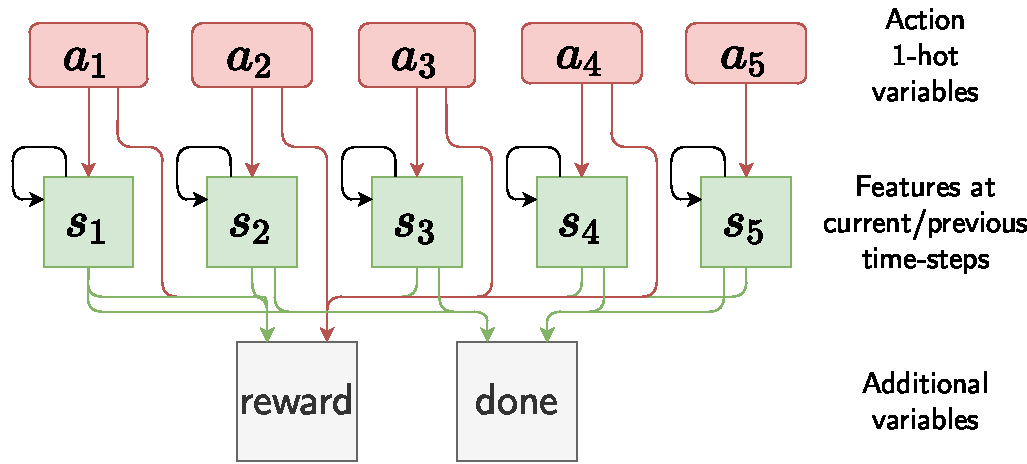
\includegraphics[width=0.7\linewidth]{diagrams/ve5_nodec}
    \caption{The causal graph for VectorIncrement$(5)$ without a decoder or an encoder. First, each state component determines its own value at the next time-step (black self-loops for $s_i$). Secondly, a corresponding action increments the state component (red line from $a_i$ to $s_i$). Finally, all state components affect reward and done (green lines from $s_i$ to reward and done), and all but one action affect the reward (red lines from $a_i$ to reward). This one of 5 possible causal graphs for this environment (one of the actions can be disconnected from the reward node). The number of edges is equal to $K(G)=24$ (out of $120$), or $K(G)=5n-1$ out of $2n^2+4n$ in the general case of VectorIncrement$(n)$}
    \label{fig:ve5nodec}
\end{figure}


\subsection{KeyChest$(h,w,f,c,k)$ environment}
The environment is described fully in my previous publication\cite{Volodin2020} at ICLR CLDM 2020.

\subsection{NonLinearSparseMatrix$(n,k)$ environment}

\section{True and learned causal graphs}
\subsection{VectorIncrement$(5)$ environment}
\subsection{VectorIncrement$(2)$ environment}
\subsection{KeyChest$(5, 5)$ environment}
\subsection{SparseMatrix$(5, 7)$ environment}

\section{Ablation study for VectorIncrement$(5)$}

\section{Failure mode analysis}

toy experiments

resulting graphs

ablation study

failure modes

In the evaluation you convince the reader that your design works as intended.
Describe the evaluation setup, the designed experiments, and how the
experiments showcase the individual points you want to prove.

This section is usually 5-10 pages.


%%%%%%%%%%%%%%%%%%%%%%
\chapter{Related Work}
\label{ch:related_work}
%%%%%%%%%%%%%%%%%%%%%%

Simple mathematical equations can describe our world well \cite{hamming1980unreasonable}. We assume that the environments in RL that we are interested in are also describable by such equations.

\cite{Battaglia2018} introduces Graph Neural Networks (GNNs) based on the idea of thoughts as graphs of connections between abstract concepts. The idea is to combine the strengths of "handcoded" or "biased" models and the "end-to-end" or "from scratch" models. \cite{Velickovic2020} extend this idea by allowing a linear (in the number of nodes) number the edges to be learned.

\cite{Cranmer2020} use GNNs to discover unknown laws of dynamics. They apply symbolic regression to the node and edge models of the GNN, to extract the symbolic expression. The model is used for pairwise forces and for discovering the laws for Dark Matter. The symbolic expression (Eureqa) generalizes better than the non-symbolic model it was extracted from. $l_1$ sparsity is used in the GNN to ease the problem for the symbolic regression.

Libraries: pytorch-geometric, graph-nets from DeepMind

\cite{Genewein} propose to use probability trees instead of graphical models to encode causal relationships. The benefit is that the set of parents of a node can be dynamically dependent on values of other nodes. The paper does not provide a way to construct the probability trees.

\cite{Zambaldi2018} introduce an attention module inside a Reinforcement Learning agent (inside the policy and the value networks), allowing it to solve tasks not solved by a simple MLP, because the task requires relational reasoning. The attention on the charts seem to favor one object attended to, corresponding to the ground truth next item to go to. Similar technique can be seen in \cite{Hahne2019} to solve visual reasoning tasks (similar to IQ tests)

\cite{Xie2020} introduce latent variables into the learned linear causal models using statistical tests.

\cite{Johnson2016} introduce a variational approach to model dynamics: probabilistic graphical model in terms of Switching Linear dynamics is applied to a learned embedding using a VAE. The model is applied to 1D and 2D image tasks, and it successfully uncovers the underlying dynamics.

\cite{VanDenOord2018} fit a neural autoregressive model. The paper suggests that fitting many-step future predictions is of utter importance, since only in such predictions the model is tested for "true" generalization of high-level features. The paper also suggests that MSE or other losses commonly used for reconstruction are not optimal, and generative models are hard to train. As an alternative, the paper suggests optimizing for the mutual information between the latent code and the original inputs. The model predicts the log-odds ratio for an offset $k$ and input up to time $t$ as $f_k(x_{t+k},c_t)\sim \frac{p(x_{t+k}|c_t)}{p(x_{t+k})}$ with a model $f_k(x_{t+k}, c_t)=e^{D(x_{t+k})^TW_kc_t}$. This model is trained using the InfoNCE loss (noise-contrastive estimation) $L=-\mathbb E_X\log\frac{f_k(x_{t+k}, c_t)}{\sum_{x_j\in X}f_k(x_j,c_t)}$. The dataset $X$ consists of one sample $x\sim p(x_{t+k}|c_t)$ (ground truth) and negative samples $x\sim p(x_{t+k})$ (the prior).

When using probabilistic inference with gradient descent-like algorithms, we need to differentiate through a sampled value $X$ with respect to the sampled parameters $X\sim X(\theta)$. For discrete distributions, reparametrization trick would not work directly, as the gradient of argmax is zero a.s. One version is the log-likelihood trick, but it results in high variance. Another approach is to replace the hard discrete distribution with a soft one, one version of which is the Concrete distribution \cite{Maddison2017}.

\cite{kalainathan2018structural, ng2019masked} propose to learn a distribution over causal graph in a mean-field way (all edges are independent and modelled as Bernoulli distribution). \cite{Brouillard2020} extend this approach to modelling interventions.

\cite{Fallah2020} use dictionary learning with an autoencoder.

\cite{kipf2019contrastive} work on learning abstract representations from pixels in 3D environments and in Atari using Graph neural networks, leading to more interpretable world (environment) models.

The related work section covers closely related work. Here you can highlight
the related work, how it solved the problem, and why it solved a different
problem. Do not play down the importance of related work, all of these
systems have been published and evaluated! Say what is different and how
you overcome some of the weaknesses of related work by discussing the
trade-offs. Stay positive!

This section is usually 3-5 pages.


%%%%%%%%%%%%%%%%%%%%
\chapter{Conclusion}
\label{ch:conclusion}
%%%%%%%%%%%%%%%%%%%%

We present the first (up to our knowledge) that learns a sparse causal graph of a Reinforcement Learning environment with a learned feature representation. We test our approach on a set of benchmarks and show a success of the proposed approach: it outputs an interpretable causal graph and allows to understand the environment. Using this approach could yield increased interpretability of Reinforcement Learning agents if used together with already existing methods requiring a causal graph as an input.

The main complexity right now is the time to fit a model of the environment, and then adjust the decoder to sparsify the model. Better (more adaptive) training procedures could speed up the convergence and increase the range of applicability of our approach.

\section{Future work}
A natural extension is to consider multiple time-step dependencies, either by stacking several subsequent observations together, or by using recurrent neural networks with structured sparsity, or by using an attention mechanism in the time axis. It would be interesting to apply our approach to natural languages and other challenging not-yet-fully-understood time series and environments such as the protein folding problem. This could yield novel insights into the latent nature of these problems.

Combining the abstract causal concept discovery with doing interventions using policies\cite{Volodin2020} using an RL agent could yield more structured exploration, and, thus, faster convergence time.


\section{Sparse causal models and the problem of consciousness}
The connection to the problem of consciousness stems comes from two directions. First, this work can be seen as an implementation of the \cite{Bengio2017} hypothesis. Indeed, we are learning the most sparse model in the latent space, along with learning the representations. The paper explicitly defines this as one of the components of the consciousness prior.


The fact that our approach works (albeit for simple environments) proves the merit of this hypothesis and shows that it could be used to explain consciousness: humans indeed can be learning abstract representations (at least partially by the virtue of) learning a space in which the dynamics becomes simple. For example, it is beneficial to learn a variable "time", because this single variable allows to predict if the sun rises, if the metro is open, or if a predator is likely to be sleeping.

Our learned representations can be used to ground the agent in natural language. Indeed, if we already have learned that there are several abstract concepts in the game such as "number of keys collected" or the "health of the player", it would suffice to only give two sentences associated with the player collecting a key or food. In contrast, a vanilla CNN given the same sentences at the same time would likely associate them with raw pixel state, and a policy network would likely associate them with the current action taken.

In this way, we shed (a bit of) light onto the easy problem of consciousness: the abstract concepts can come {\em before} language, in an unsupervised way, and the first words of language are simply mapped to already existing concepts using Hebbian learning (word and the stimulus occur together). Next, this process could be bootstrapped, since presence of words becomes new variables in the causal model, and the process is repeated, with a more powerful model and a more powerful set of words learned. Asking questions like "what is X?" can be seen as performing interventions on the causal graph: we know that asking "what is X" is likely to result in novel data (a learned way to optimize for an objective), and an $X$ is a novel variable which is still largely unused. Therefore, the agent intervenes setting $\mbox{do}(\mbox{ask 'what is X'})$ and samples data from a novel distribution.

While the grounding technique is known for a long time, my work provides a proof that abstract concepts can be learnt before language from raw pixels, just by optimizing for the inner model simplicity -- a simple and beautiful enough principle to be innate to the brain. Other projects like mine are involving more sophisticated (and less simple) priors, such that the action only increments one component, or that the dynamics in the latent space is linear, or that the environment is a $2D$ world.

Secondly, I express a hypothesis that a learned representation is crucial when dealing with the Integrated Information Theory. Currently, the theory does not seem to specify at which level of abstraction it should be applied -- at the level of atoms, or at the level of molecules? Or, maybe, at the level of individual electrical components of a computer that we examine? Specifically, it is unclear what should be the "nodes", "factors" or "variables" in the model, the dependencies between which we are to examine to compute the $\varphi$. This leads to the value of $\varphi$ potentially being arbitrarily high, if a bijective transformation is applied before the analysis [epfl paper].

If we declare that we need to first apply a transformation in which the graph becomes most sparse (which intuitively is connected to the value of $\varphi$: a sparse graph will likely have less edges, or even becomes two independent components instead). Next, we compute $\varphi$. This seems to resolve the issue raised in [epfl paper], albeit, in a bit of an ad-hoc fashion. More importantly, this resolves the ambiguity of the level of abstraction the theory should be applied: if we apply a decoder first and optimize for sparsity (or, maybe, low $\varphi$), the raw wave-function can be mapped into the state of molecules -- and the two are (somewhat) bijective.

Because of this connection between $\varphi$ and sparsity, our approach can be seen as approximately computing the $\varphi$ for the {\em environment}, in other words, how conscious it is. With this in mind, the VectorIncrement environment, for example, is not conscious: its causal graph is a union of two connected components (the "done" and the "time" is not connected to everything else), but can be seen as two "conscious" components. In contrast, the KeyChest environment's graph has only one connected component, and, thus, potentially has a non-$0$ $\varphi$ as a whole. However, this claim does not seem to be empirically testable, at least now.

% Appendices are optional
% \appendix
% %%%%%%%%%%%%%%%%%%%%%%%%%%%%%%%%%%%%%%
% \chapter{How to make a transmogrifier}
% %%%%%%%%%%%%%%%%%%%%%%%%%%%%%%%%%%%%%%
%
% In case you ever need an (optional) appendix.
%
% You need the following items:
% \begin{itemize}
% \item A box
% \item Crayons
% \item A self-aware 5-year old
% \end{itemize}

\chapter{OLD text, to copy-paste and remove}
\section{Introduction}
Consciousness prior, AIXI lead to simple or sparse models.

Disentangled representations and representation learning

Model-based reinforcement learning

Causal modelling for reinforcement learning. Interventions

AI safety: distributional shift robustness (generalization), interpretability, sample-efficiency

\section{Proposed architecture}
\subsection{Theory}
Like in AIXI, would like to find the simplest model of the environment:
$K(\mu)\to\min$ s.t. $L(\mu, data)\to\min$. In general, this problem is uncomputable.

We decompose the model into a Decoder and a sparse Model. The model in observational space $W$ is then the sparse Model $M$ applied to Decoded features, with the result projected back into the high-dimensional space.
$$
W=D^{-1}MD
$$

\subsubsection{Why sparse models?}
Traditionally, sparsity of models usually means making the number of non-zero parameters low. This can be seen in linear regression when applying the Lasso regularization. Such methods learn to rely only on a handful of features, instead of considering the whole input. When data is multicollinear, this leads to better generalization, as the model only relies on the most salient features, and is less likely to learn spurious correlations between features.

In Supervised Deep Learning, sparsity of representation traditionally means regularizing the activation of the latent hidden layer in an autoencoder-like setup (an encoder transforming a high-dimensional representation into a low-dimensional one, and then a decoder doing the inverse transform back to the high-dimensional space). In such setups, sparsity is enforced in order to enforce constraints on the learned latent space. With such regularization, the model is learning a sparse coding -- one where each input is represented with a minimal number of non-zero components.
This representation is better than a "dense" one, in case if there are certain regularities in the dataset.
For example, if the input images have an underlying latent generative model in which the high-dimensional image is a "child" of only few discrete variables (such as, a cat can only be of certain colors, which can be represented in a one-hot way, and other images, such as images of dogs, can be distinguished from images of cats by another binary variable).
In neuroscience, such representations are biologically plausible due to lower energy usage and higher fault tolerance [??].

However, sparse representation does not necessarily imply interpretability. In supervised tasks, it it known that [Google post on disentanglement] the model still learns spurious correlations, which leads to different controllable aspects of the image being "entangled" in one activation node.

Spurious correlations in supervised learning do not have a general way of being resolved, because observational data is not enough to learn the correct causal model. An example of this is adversarial images, which can be seen as spurious correlations, namely, the model relying on high-frequency features which, while discriminating between images on the training set due to high memorizing capacity of the network, do not generalize to the shifted adversarial distribution [features not bugs post].

While the problem of learning good models from observational data is interesting in its own right, in this project we focus on a reinforcement learning setting where there is a possibility to perform actions. Since switching from one policy to another determines the distribution of histories, switching from one policy to another can be seen as performing interventions on the underlying causal graph. In this way, for example, an agent playing Breakout by precisely targetting each block one-by-one is different from an agent trying to put the ball to the top of the playing field, speeding up the process significantly. If we consider the underlying data generation process in the latent space of positions of various objects (x and y coordinates of the ball, the player and all the targets), and in an interaction between them, and a similar representation for the agent (for example, the first agent's action depends on the leftmost still-standing target, which it hits perfectly, and the second agent's action depending as well on whether or not there is an opportunity to get to the top), switching from one policy to another can be seen as an intervention in this history-generating graphical model, in which the gate switching the dependencies of the policy's action is altered, and set to $1$ instead of $0$, signifying the reliance to the second strategy.

While the total space of policies is represented with exponentially many such switch nodes (namely, one node for each subset of coordinates the policy can possible depend on, and one node for every discretized value of the weights of a neural network, for example), some of them are more complex than others.

We start the theoretical derivation from the AIXI framework, where the environment is a Turing machine, and the agent is a non-computable greedy best-response Bayesian solution considering all possible environments. Theoretically, such agent is known to have certain optimality conditions under the assumption of sufficient exploration. Compared to Solomonoff  induction (a perfect uncomputable Bayesian solution to the online supervised learning problem, or the task that the GPT-3 solves -- self-supervised prediction), in RL, AIXI (which is designed in the same way as the Solomonoff induction) is not always optimal. Indeed, it was discovered that AIXI does not explore enough, because there are bad priors leading to the agent "believing" that it is not beneficial to explore. In the simplest setting, we can always select such a prior where the probability of the true environment, and of any sufficiently close-by environment leading to rewards when taking action $a_1$ is arbitrarily low, leading to the agent never trying $a_1$, and, thus, never updating its posterior [On the optimality...].

General theory of RL suggests solutions to this problem, leading to weaker convergence results [Thompson sampling]. The basic idea is to let go of the agent being perfectly Bayesian, and (knowingly) use an outdated model to take actions. Intuitively, this 'denial' leads to even improbable actions being taken into consideration, and, thus, has more chances of discovering the true posterior.

The Solomonoff Bayesian setting considers weighting the environment models by their complexity.

In this setting, we consider the prior over environments $\mu$, $\xi(\mu)=2^{-K(\mu)}$ where $K$ is the Kolmogorov complexity. Next, we collect history using a policy $\pi$, which gives a Bayesian posterior:

$$
\nu(\mu|h)=\frac{\mu(h)2^{-K(\mu)}}{\sum_{\nu}\nu(h)2^{-K(\nu)}}=\frac{\mu(h)\xi(\mu)}{\xi(h)}
$$

Given the posterior $\nu'=\nu|h\equiv \nu(\mu|h)$, we "simply" run an infinite tree search to find the best possible action:
$$
a_t^{AIXI}=\arg\max_{a_t}\sum\limits_{t=t_0}^{\infty}\gamma^t\sum_{r_t,s_t}\nu'(r_t,s_t|r_{<t}s_{<t}a_{<t})
$$

Here, $\xi(h)$ is the prior probability of the data, or the probability of history in the Universal Environment (a mixture of environments where each environment is weighted with its complexity).

In practice, it is not viable to search over all possible Turing machines (which is required to evaluate the denominator, $\xi(h)$), and we cannot run them for an infinite number of time-steps (like it is done in AIXI). Another problem here is that we cannot compute $K(\mu)$.

To make the problem practical, we additionally assume that there is a structure to the environment.

Namely, we assume that for the whole environment there exist a mapping $f\colon o\to f$ which maps observations to features. For a while, we assume deterministic environments. We also assume 1 time-step dependencies (Markov property). Given our feature assumption, we assume that in the feature space, the dynamics of the environment is linear (inherent simplicity??). We only consider environments $\mu$ which are representable (we consider $r_t$ as part of $s_t$ for simplicity of notation here) as
$$
f_t(\mu)=M_ff_t+M_aa_t+b
$$

{\bf OMG}





Here, $f_t=D(s_t)$ and $s_t=R(f_t)$

Imagine if the representation $f$ is sparse at every time-step. Does this guarantee an interpretable environment?

From the point of view of the Free Energy principle, we are looking for a minimal Markov Blanket.

From the point of view of the leading theory of consciousness, Integrated Information Theory. Why do we look for sparsity, when consciousness there is about irreducibility of a big model into smaller models? IIT does not specify which representation of the physical world needs to be mapped to the nodes in the causal graph, while we have a decoder which learns this representation, and selects one where the model is the simplest one. Tononi says that we should pick the representation with maximal $\phi$, but, it seems, In our case, something not affecting the reward (or the reconstruction in general), would be independent of causal variables that are optimized for. Thus, such a variable would be unconscious. The project can be seen as computing a proxy for $\phi$ -- minimizing the complexity. Such an interpretation of IIT (allowing for an arbitrary function computing the representation, and minimizing over complexities/$\phi$) could resolve the issues raised in \cite{doerig2019unfolding}. There, a function is applied to the representation, after which an inverse transform is applied. If we only care about the minimal-$\phi$ representation, all of that would be cancelled, and only the high-level variables would remain.


What if the decoder is too complex? We could re-use components, like humans don't need to re-learn existing conv1 filters to learn a new game.

In the model, we can sample from a categorical gumbel-softmax distribution in order to select a model. We can re-use models for different features. Each of the feature models has a categorical distribution over the bank of models, and we regularize for the total entropy of all models (with an addition that we can permute the features in arbitrary way before applying the model).


The total complexity of the environment $\mu$ is thus $K(\mu)=K(M_a)+K(M_f)+K(D)+K(R)$


$\mu(h)\equiv \mu()$

Finding good features by regularizing the {\em model} to be sparse.

Three losses: model fit, sparsity regularization, reconstruction

Reconstruction losses: inverse decoder norm, reconstructing observations (autoencoder), inverse model norm (we force the model to be an invertible matrix), predicting actions, predicting value function from features (like in muzero)

Causal learners: linear, graph NNs, linear with sampling

For the model fit, we use Mean Squared Error. Alternatives are to use contrastive loss (with fake samples)

For the sparsity, we use L1-regularization. An alternative is to use projection.

Architecture improvements: model at each layer of the decoder for a faster fit, many time-steps, batch normalization, adaptive sparsity loss



\section{Model learning for a fixed policy}
The problem of learning a model is formulated as follows. Given a deterministic RL environment $\mu$ and a policy $\pi$, we want to find a function computing the next observation: $o_{t+1}=M_o(o_t, a_t)$. Additionally, we would like to learn the reward and the termination ("done"): $r_t=M_r(o_t, a_t)$, $d_t=M_d(o_t, a_t)$. Since observations are high-dimensional, we require the model to be represented as a composition of a decoder, a model in the feature space, and a reconstructor: $o_{t+1}=R(M_f(D(o_t), a_t))$. If we denote $f_t=D(o_t)$, we can additionally require $D(o_{t+1})\approx M_f(f_t, a_t)$. In this case, the function $M_f$ is a {\em model in feature space}. If we additionally require $R(D(o_t))\approx o_t$, the function $R$ becomes the inverse for the decoder.

Training the reconstructor is usually the most time-consuming part, since it requires to train a generative model for high-dimensional observations. Therefore, several techniques are applicable to avoid this part. In these cases, a full model in observation space is not obtained.
\begin{enumerate}
    \item Margin loss in the space of observations. For observations $o_1\neq o_2$, we require that $\rho(D(o_1), D(o_2))\geq h$ via a margin loss: $\max(h-\rho, 0)\to\min$
    \item Contrastive loss: we train a classifier $C(f, f')$ with a loss $\frac{C(f_t, f_{t+1})}{C(f_t, f_{t+1})+C(f_t, f_{neg})}\to\max$ where $f_{neg}$ is not equal to the true feature $f_{t+1}$
    \item Training a discriminator with labels $C(f_t, f_{t+1})\approx 1$, $C(f_t, M_f(f_t, a_t))\approx 0$, and with a separate optimizer training for $C(f_t, M_f(f_t, a_t))\approx 1$ (GAN)
    \item Instead of predicting high-dimensional observations, only predicting some sufficient (in the sense of playing the game) statistic, such as the value function: $V_f(D(o_t))\approx V(o_t)$, where $V_f$ is a trainable value-to-go predictor, and $V(o_t)$ is the reward-to-go collected at the episode.
\end{enumerate}

{\bf Sampling procedure.} Since we would like the model to approximate the next observation $o_{t+1}\approx M_o(o_t, a_t)$, we must sample triples $(o_{t+1}, o_t, a_t)$ (and other related features such as reward, termination, or reward-to-go) from the uniform distribution: we randomly sample an episode, and then pick a random observation. This would mean that we only keep one step from a whole episode. This is not practical, as we have to "throw away" most of the steps. We approximate this with an experience replay buffer. In case if the environment "looks differently" for different initialization random seeds (for example, the labyrinth has a different layout), such an approximation results in the following issue. If we sample a mini-batch from 1 episode, and the subsequent mini-batch from another (single) episode, the model would tend to overfit to the first mini-batch (specifically, for example, to the locations of objects in the labyrinth). On the next call, the loss will spike, and the model will overfit to the next object locations. Having an experience replay buffer and sampling the triples randomly from it alleviates the issue. This is the same problem as was encountered in the DQN paper.

In practice, we use the mean-squared regression. To account for different scales of observation components, feature components and rewards, we compute the {\em relative} mean absolute error:
$$
L_{rel-mse}(f^{pred}, f^{true})=\frac{1}{T}\sum\limits_{t=1}^T\sum\limits_{f=1}^F\left[\frac{f^{true}_{f,t}-f^{pred}_{f, t}}{\sigma'(f^{true}_{f, \cdot})}\right]^2
$$

Here $\sigma(f^{true}_{f, \cdot})$ is the standard deviation for the true features. In case if this value is less than $\varepsilon=10^{-8}$, we set this value to $1$. This is required for the case of constant pixels, or constant features. Setting this value to $\varepsilon$ instead of $1$ produces extremely high loss spikes in case if in some of the batches, a feature is constant, and in others, it is not.

The relative loss $L_{rel-mse}$ is more interpretable than the standard mean-squared-error loss, because its value signifies how many features have a large error. For example, for $10$ equal features with equal predictions, a value $L_{rel-mse}=10$ means that for all features, the prediction error is equal to the standard deviation. More importantly, a value $L_{rel-mse}=10^{-2}$ means that for each of the features, the relative error is at most $10\%$ in terms of the standard deviation.

\begin{itemize}
    \item Reconstruction loss: $L_{rec}=L_{rel-mse}(R(D(o_{x})), o_{x})$. Here we denote values before (and while) taking an action as $x$, and values at a step immediately after taking an action as $y$. In this notation, for example, $o_{x, t+1}=o_{y,t}$
    \item Prediction loss in observation space: $L_{pred}=L_{rel-mse}(R(M_f(D(o_{x}, a_{x})), o_{y})$
    \item Feature consistency loss in feature space: $L_{cons}=L_{rel-mse}(M_f(D(o_x, a_x)), D(o_y))$
\end{itemize}

Both of the losses $L_{pred}$ and $L_{cons}$ are required to obtain good features. First, training with $L_{pred}$ allows to have an end-to-end model, where the right-hand side does not depend on the decoder. This becomes a supervised learning problem. Secondly, without optimizing for the feature consistency loss, $L_{pred}=0$ does not guarantee that $L_{cons}=0$, since the reconstructor can "recognize" two different sets of features. In this case, output features from the model do not necessarily correspond to the input features.

Since we would like to obtain an interpretable model, we add the feature consistency loss $L_{cons}$.

{\bf Separate models for each feature and each pixel.} Empirically, in our test toy environments (VectorIncrement and KeyChest), the tasks of predicting different pixels with a reconstructor $R$ do not have many information in common, and, therefore, are poor tasks for multi-task learning. Empirically, predicting each pixel $i$ with a separate model $R_i(f)$ converges faster than having a joint neural network $R(f)$.

\section{Sparse model learning}
Suppose that we have reasonably low losses $L_{rec},\,L_{pred},\,L_{cons}<\varepsilon$. This means that for each of the output pixels, we can predict it with relative error at most $\varepsilon$. In addition, the same applies to the relative error in predicting each feature.

In the space of all reconstructors, decoders and models, we would like to find a model which is most sparse in the sense of a causal graph. This means that, for each output feature $f_j$, we would like it to depend on the fewest amount of input features $f_i$. Given that, the graph of dependencies in the feature space is most sparse (in terms of the number of edges), or, the program describing the environment is most simple.

To do so, we use the model from Bengio. We use a tensor of probabilities of shape $p=(F+F', F+A)$, where $F$ is the number of features, $F'$ is the number of additional features to predict (2 -- reward and termination), and $A$ is the number of actions. This tensor has values between $0$ and $1$. The values are interpreted as probabilities of having an edge from feature $f_i$ to feature $f_j$: if the value is $1$, the feature $f_j$ depends on $f_i$ with probability $1$.

Given such a tensor of probabilities, we can sample random variables $\xi\sim p$, where $\xi$ is a binary matrix of dimensions $(F+F', F+A)$ with values in $\{0, 1\}$. Now, if an edge is not present in the graph, the model for a feature should not depend on the corresponding input feature. We achieve this by multiplying the input with this tensor $\xi$. Next, we have $F+F'$ models predicting each feature, each depending on the input multiplied with the binary mask $\xi$.

Having $F+F'$ independent models instead of having one big model with $F+F'$ outputs has the same advantage as stated before for the reconstructor $R$: since the tasks do not have a lot in common, the convergence is faster if the networks are independent.

In addition, the model receives the mask $\xi$ apart from the input $[f_t, a_t]\odot \xi_i$. This is necessary because the model needs to "know" whether it has received $0$ as input because the feature is $0$, or because the feature was "de-selected".

Suppose that we have a dataset of triples $\{(f_{t+1}, f_t, a_t)\}$. We sample masks $\xi_t$ for every time-step $t$. For this example, we set $p_{ji}=0.5$ for all features. The loss $L_{pred}$ and $L_{cons}$ becomes a random variable, because the inputs a pre-multiplied by random masks. If we fit the model on this data (in a supervised way), it will learn to rely on features if they are present, and to replace them with a "mean value" in case if they are not. We can optimize the parameters of $R, M, D$ using gradient descent. Now, how to obtain the gradient with respect to $p$?

The well-known trick is Gumbel-Softmax, which can yield $\frac{\partial L}{\partial p}$ given samples. However, since it internally uses saturating softmax,  it takes a lot of time in practice to obtain a value close to $1$. Even in the mostly-linear regime, it takes a lot of time to optimize for parameters $p$, because the gradient is multiplied by $\sigma(\cdot)(1-\sigma(\cdot))$. Instead, we use the REINFORCE gradient:

$\frac{\partial L}{\partial p}=\frac{\partial}{\partial p}\mathbb{E} L(\xi(p))=\frac{\partial}{\partial p}\mathbb E_{\xi_{11}}...\mathbb E_{\xi_{nm}}L(\xi_{11},...,\xi_{nm})$.

Now, consider one-dimensional case and $\frac{d}{dp}\mathbb E_{\xi\sim F(p)}L(\xi)=\int \frac{d}{dp}f_p(\xi)L(\xi)d\xi$. Now, using the log-likelihood trick, $\frac{df_p(\xi)}{dp}=\frac{d\log f_p(\xi)}{dp}f_p(\xi)$. Therefore, $\frac{d}{dp}\mathbb E_{\xi\sim F(p)}L(\xi)=\int\frac{d\log f_p(\xi)}{dp}f_p(\xi)L(\xi)d\xi=\mathbb E_{\xi\sim F(p)}\frac{d\log f_p(\xi)}{dp}L(\xi)$. In case of discrete distributions, we need to replace the probability density function $f_p(\xi)$ with the probability mass function $F_p(\xi)$

For the Bernoulli distribution, this gives $\frac{d}{dp}\mathbb E_{\xi\sim Be(p)}=\sum_{\xi\in\{0, 1\}}\frac{d\log F_p(\xi)}{dp}L(\xi)$. Since $F_p(1)=p$ and $F_p(0)=1-p$, we obtain $\frac{d}{dp}\mathbb E_{\xi\sim Be(p)}=L(\xi=1)-L(\xi=0)$.

In case if we have many random variables $\xi_{ji}$, we can set $L(\xi_{ji})=\mathbb E_{\xi_{-ji}}L(\xi_{ji}, \xi_{-ji})$, and then obtain $\frac{\partial }{\partial p}L_{rel-mse}=\mathbb E_{\xi_{-ji}}L_{rel-mse}(\xi_{ji}=1, \xi_{-ji})-\mathbb E_{\xi_{-ji}}L_{rel-mse}(\xi_{ji}=0, \xi_{-ji})$.

In practice, given a sample of $\xi$ of shape $[T, F+F', F+A]$, for a pair of features $j, i$, we select the values of the loss $L_{t}$ where $\xi_{t, j, i}=1$, and take the average of such $L_t$ to obtain a sample estimate of $\mathbb E_{\xi_{-ji}}L_{rel-mse}(\xi_{ji}, \xi_{-ji})$. The same procedure is applied for the values of $t$ where $\xi_{t, j, i}=0$. This corresponds to running $F+F'\times F\times A$ "randomized control trials" to establish the effect of $\xi_{ji}$ on $L$, and computing the difference in means. This way, we manually compute the gradient for each $p_{ji}$.

While REINFORCE gradients are known to be noisy, here we only have two values, and sample sizes are considerably large for large batch sizes $T\sim 5000$ and $p\sim 0.5$. By the central limit theorem, the sample means are close to the true expectations. After applying the gradient, the probabilities $p$ are clipped to be between $0$ and $1$.

Note that the problems of estimating the gradient are not independent, in a sense that a gradient with respect to $\xi_{ji}$ depends on values of $p_{-ji}$. This happens because the values of the loss depend on these features as well.

To turn the features off, we introduce a sparsity regularizer. To ease this even more, we add a version of the losses with $p=0.5$ (regardless of the true value of $p$). To train the model faster, we add a version of the loss with $p=1$ as well.

Denote $L_{model}=L_{pred}+L_{cons}$. Given the two other versions with $p=0.5$ and $p=1$ we have also $L_{model}^{p=0.5}$ and $L_{model}^{p=1}$.

\subsection{Annealing.} To learn a sparse model, we additionally regularize the probabilities $p$ for sparsity as $L_{sparse}=\sum_{ij}|p_{ij}|$. The total gradient for $p$ is a sum of gradients from $L_{sparse}$ and the REINFORCE gradient from $L_{pred}$ and $L_{cons}$.

Consider the relative error ("relative sparsity gap") $\gamma(R, D, M, p)=\frac{L_{model}^{p=p}-L_{model}^{p=1}}{L_{model}^{p=p}}$. It shows how the loss given the current selected features compares to enabling all features. For a any fixed $p$ and any $D$, if we fit the $M$ and $R$ on $L_{model}$ and $L_{model}^{p=1}$ (note that there is no conflict between these two losses, because masks uniquely determine whether the features are on or off. Essentially, this is a big supervised dataset), the value of $\gamma\in[0, 1]$: turning off some features can only increase the loss. In case if $p<1$ and $\gamma=0$, the output does not depend on the input. If $\gamma=1$, the model perfectly fits the data ($L=0)$ with $p=1$ (this does not happen in practice). $\gamma=0.5$ means that the error could decrease $50\%$ in case if we turn on all features.

An additive error $\delta(R, D, M, p)=L_{model}^{p=p}-L_{model}^{p=1}$ is in range between $0$ (if model is trained) and $N=F+F'$ (in case if model can perfectly fit the data and $p=0$). Therefore, we consider the ratio $\Delta(R, D, M, p)=\frac{\delta(R, D, M, p)}{F+F'}\in[0, 1]$.

Annealing proceeds in the following stages:
\begin{enumerate}
    \item $\delta>\delta_{\max}$. In this case, the model is trained to decrease $L_{model}^p$, which increases some $p$. Sparsity coefficient is decreased (we care more about fitting any model rather than about sparsity).
    \item $\delta\leq \delta_{\max}$. In this case, we care about sparsity and increase the coefficient. In case if at some point, $\delta$ crosses the threshold, we do not change the coefficient for some time, to allow the model to learn from a dataset where some features are turned off. This "freezing" at a "low temperature" allows the model to "crystallize" and learn a new representation (one where some features are turned off).
\end{enumerate}

Consider the following cases:
\begin{enumerate}
    \item $p=p_{\min}$. In this case, the model cannot predict features reliably: even in the toy example above, the error would be $L\sim 2\times (1-p)\approx 2$ for 2 features -- very bad result for a relative error. In this case, the REINFORCE gradient will turn on features yielding maximal decrease in the loss.
    \item $p=1$. In this case, we would like to turn off some of the features, because we would like to obtain the most sparse model.
\end{enumerate}

Overall we would like to find the sparsest graph such that the sparsity gap does not exceed some $\varepsilon_{\max}$:
$$
\min L_{sparse}\,s.t.\,\delta\leq \varepsilon_{\max},L_{model}^{p=1}+L_{rec}\leq \varepsilon_{loss}
$$

This is a constrained optimization problem. There are several approaches to this problem:
\begin{enumerate}
    \item Static linear combination: $\frac{L_{sparse}}{NM}+\frac{L_{model}^{p=p}+L_{model}^{p=1}}{2N}+\frac{L_{rec}}{O}$
    \item Dynamic linear combination: $\frac{L_{rec}}{O}+\frac{L_{model}^{p=1}+L_{model}^{p=p}}{2N}+\beta L_{sparse}$ where $\beta$ is chosen based on the value of $\delta$ as described above
    \item Lagrange multipliers. We consider $\mathcal L(\lambda, D, M, R)=L_{sparse}+\lambda (L_{rest}-\varepsilon_{rest})$. The point with $\max_{\lambda}\min_{D, M, R}\mathcal L$ corresponds to $L_{sparse}\to\min$ s.t. $L_{rest}\leq\varepsilon_{rest}$. The standard solution is a primal-dual method:
    $$\lambda_{t+1}=\lambda+\eta\frac{\partial \mathcal L}{\partial \lambda}$$
    $$(D, M,R)_{t+1}=(D,M,R)-\eta\frac{\partial\mathcal L}{\partial (D, M, R)}$$
\end{enumerate}

\section{Environments}
\begin{enumerate}
    \item VectorIncrement. Recovering a sparse linear matrix from skewed observations
    \item KeyChest. Learning a sparse causal graph in a grid-world
    \item Physics environments. Learning physics laws
    \item Atari: MsPacman, Montezuma Revenge. Learning a better representation than pixels
    \item PyGame learning environment (flapping bird)
    \item Starcraft. Learning in high-dimensional environments
    \item VIZDoom. Learning abstract features
    \item TextWorld. Extracting a low-dimensional model governing the decisions
    \item OpenSpiel. Finding good representations automatically for known games
\end{enumerate}

\section{Results}

\begin{enumerate}
    \item Can fit a sparse model on VectorIncrement with pinverse sparsity loss, fully-connected nets and value function for reconstruction
    \item Can train agent on KeyChest (DQN and PPO) demonstrating that it is Markov
    \item Can fit a sparse model (without sparsity regularization) ignoring actions that somewhat well predicts the health (but not health increase, only decrease)
    \item Cannot fit a VAE, AE, VAE-GAN on KeyChest data for some reason
\end{enumerate}

\subsection{What does MuZero learn}
\subsection{Learned graphs for our environments}
\subsection{Game complexities}
\subsection{Properties of the new agent}
\subsubsection{Spurious correlations and exploration speed}
\subsubsection{Sample efficiency}
\subsubsection{Online DS robustness (re-training speed)}
\subsubsection{Offline DS robustness (deploying into the environment)}

\cleardoublepage
\phantomsection
\addcontentsline{toc}{chapter}{Bibliography}
\printbibliography

\end{document}
